\documentclass[../Main.tex]{subfiles}

\begin{document}

\chapter{Metric Spaces}

\section{Fundamental Definitions n' Stuff}
\defn{Metric Space}{A set $X$ along with a function $d:X \times X \to \RR^{+} \cup \{0\}$ called distance, is said to be a metric space if: \begin{enumerate}
    \item $d(x,y)=0 \iff x=y$ (Positivity)
    \item $d(x,y)=d(y,x), \forall x,y \in X$ (Symmetric)
    \item $\forall x,y,z \in X$ we have, $d(x,y) \leq d(x,z)+d(y,z)$ (Triangle Inequality)
\end{enumerate}}
\exm{$\RR^n$ as a metric space}{Note that $\RR^n$, the set of all n-tuples of $\RR$, is a metric space with $$d(\vec x,\vec y):=|\vec x-\vec y|= \sqrt{(x_1-y_1)^2+(x_2-y_2)^+\cdots+(x_n-y_n)^2} $$}
\defn{Open and Closed Balls around $x$ in $X$}{Open ball is defined as: $$B_{r}(x):=\{y \in X:d(y,x)<r \}$$
\\\\ Closed ball is defined as: $$ B_{[r]}(x):=\{y\in X:d(y,x) \leq r\}$$}
\defn{Convexity}{A set $S$ in $\RR^n$ is said to be convex if $\forall x,y \in S, t \in [0,1]$, $x+t(y-x) \in S$}
\exm{Open and closed balls in $\RR^n$ are convex}{Consider $B_r(x):=\{z \in \RR^n: |z-x|<r \}$. Consider arbitrary $p$ and $q$ in $B_r(x)$. We have that $d(p,x)<r$ and $d(q,x)<r$. Consider $p+t(q-p)$ and consider $d(p+t(q-p),x)=|p+t(q-p)-x|=|tq+(1-t)p-x+tx-tx|=|tq-tx+(1-t)p-(1-t)x|\leq t|q-x|+(1-t)|p-x|=td(q,x)+(1-t)d(p,x)<r$. Replacing $<$ with $\leq$ in the above proves the result for closed balls.

}
\defn{Sequences in Metric Spaces}{A sequence $\{x_n: x_n \in X\}$ is a mapping from the naturals to $X$, where order is implicit. We say a sequence in a metric space $X$ is convergent to $x \in X$ if: $$(\forall \varepsilon>0)(\exists n_0 \in \NN)(\forall n \in \NN, n \geq n_0)(d(x_n,x)<\varepsilon)$$}
\defn{Limit Point of a set $E$}{We say $p$ is a limit point of a set $E$ if $$(\forall \varepsilon>0)(\exists q_{\varepsilon} \in E; q_{\varepsilon} \neq p)(d(q_{\varepsilon},p)<\varepsilon)$$ In other words, in every $\varepsilon$-ball around $p$, there would exist a point $q_{\varepsilon}$ in $E$, which is different from $p$.  }
\thmp{}{Every ball / neighbourhood of $p$ which is a limit point of $E$, would contain infinitely many points $q$ such that $q \in B_{\varepsilon}(p) \cap E\setminus \{p\} $}{Suppose for some neighbourhood, there only exists finite points $q_1,q_2,\cdots q_k$ such that $q_j \in B_{\varepsilon_0} \cup E\setminus\{p\}$. Let $\delta<min\{d(p,q_j): j \in [1,2,...k]\}$. We then have that, there exists no point $q \in E$ such that its distancce from $p$ is less than $\delta$, making $p$ a non-limit point. Absurd.}
\cor{A finite set has no limit points}
\thmp{Recharacterisation of Limit points}{A point $p \in X$ is a limit point of $E \subset X$ if and only if there exists a sequence $x_n \in E$, $x_n\neq p \forall n \in \NN$ such that $\{x_n\} \to p$}{$\implies$) If $p$ is a limit point, around every neighbourhood, there would exist a point $q_\varepsilon \in E$ such that $0<d(q_\varepsilon,p)<\varepsilon$. Choose $\varepsilon_1=1$, and obtain $x_1$ such that $x_1 \in E$, $x_1 \neq p$ and $0<d(x_1,p)<1$. Choose $\varepsilon_2=\frac{1}{2}(d(x_1,p))$. We find $x_2 \in E$, $x_2 \neq p$ such that $d(x_2,p)<\frac{d(x_1,p)}{2}<\frac{1}{2}$. Continue as such to obtain a sequence that converges to $p$.
\\\\ $\impliedby$) Suppose there is a sequence $x_n$ such that $x_n \neq p \forall n \in \NN$ and $\forall \varepsilon, \exists n_0(\varepsilon)$ such that $\forall n \geq n_0$ we have $d(x_n,p)<\varepsilon$ which means for a given $\varepsilon$, there exists a point $x_{n_0+1}$ in $E$ such that it is not equal to $p$ and it is in the $\varepsilon$-ball of $p$. Hence, $p$ would be a limit point. }
\defn{Closed sets in $X$}{A set $E$ is closed in $X$ if every limit point of $E$ is contained in $E$}
\defn{Equivalent definition of closed sets in $X$}{A set $E$ in $X$ is closed if for every convergent sequence $x_n$ in $x$ such that $lim(x_n) \neq x_n$ for any $n$, we have $lim(x_n) \in E$.}
\defn{Open sets in $X$}{A set $E$ is said to be open if $\forall x \in E$, $\exists \xi_x>0$ such that $B_{\xi_x}(x) \subset E$}
\thmp{}{Every open ball is an open set}{Suppose $a$ is a fixed point in $X$ and $\delta>0$ is given. $B=B_{\delta}(a):=\{y \in X: d(y,a)<\delta\}$.Consider arbitrary $z \in B$, for which we have $d(z,a)=t<\delta$. Therefore $\delta-t>0$. Consider $0<\xi_z=r<\delta-t$ from Density. Consider an arbitrary $x$ such that $d(x,z)<\xi_z=r<\delta -t$. $d(x,a)\leq d(x,z)+d(a,z)=r+t\leq \delta -t+t=\delta$. We are done.}
\defn{Compliment with respect to $X$}{If $E \subseteq X$, we define compliment of $E$ as $$E^C:=\{ x\in X:x \not\in E\}$$}
\defn{Bounded}{A set $E \subset X$ is bounded if $\exists$ a positive number $M>0$ and $q \in E$ such that $d(x,q)<M$ $\forall x \in E$. i.e, all the points of $E$ gets contained in some ball in $X$. }
\thmp{De Morgan's Law}{Let $\{E_{\alpha}: \alpha \in A\}$ where $A$ is some arbitrary indexing set represent a collection of sets in $X$. Then $$(\Bigg.\cup_{\alpha} E_{\alpha})^{C}=\Bigg.\cap_{\alpha}E^C_{\alpha}$$}{Consider $(\cup_{\alpha} E_{\alpha})^c=\{x \in X: \exists \alpha \in A: x \in E_{\alpha} \}^c=\{x \in X: \forall \alpha \in A: x \not\in E_{\alpha} \}=\{x \in X: \forall \alpha \in A: x \in E^c_{\alpha} \}=\cap_{\alpha}E^c_{\alpha}$}
\thmp{The Big Equivalence}{$E \subset X$ is open $\iff$ $E^c$ is closed.}{
$\implies$) Suppose that $E$ is open but $E^c$ is not closed. This means that there exists a limit point of $E^c$ that falls in $E$, i.e, outside $E^c$. Let this be $q$. This means for every $\varepsilon$-ball around $q$, a point of $E^c$ exists. But since $E$ is open and $q\in E$, we have for a particular $\varepsilon$-ball, inside which, no point of $E^c$ resides. Contradiction.\\\\
$\impliedby$) Suppose $E$ is closed but $E^c$ is not open. This means that there is a point in $E^c$, $p$, such that for every $\varepsilon$-ball around $p$, some point in $E$ falls into this ball. But this makes $p$ a limit point of $E$, which is absurd since $E$ is closed, limit points fall into the sets themselves.
}
\thmp{}{For a collection of open sets $\{G_{\alpha} :\alpha \in A\}$, $\cup_{\alpha} G_{\alpha}$ is also an open set.}{Consider $x \in \cup_{\alpha} G_{\alpha}$ which means $\exists \alpha_x \in A$ such that $x \in G_{\alpha_x}$ which means, there would exist an $\xi$-ball around $x$ that is contained in $G_{\alpha_x}$ which is in turn contained in $\cup_{\alpha} G_{\alpha}$.}

\corp{For any collection of closed sets $E_{\alpha}$, $\cap_{\alpha} E_{\alpha}$ is also closed.}{$\{ E^c_{\alpha}\}$ is a collection of open sets, and $\cup_{\alpha} E^c_{\alpha}$ is an open set, which means $\cup_{\alpha}E^c_{\alpha}=(\cap_{\alpha} E_{\alpha})^c$ is an open set, from which we get that $(\cap_{\alpha} E_{\alpha})$ is a closed set.}

\thmp{}{For any finite collection of open sets $\{E_1,E_2,\cdots E_k\}$, $\cap_{i=1}^kE_i$ is also open.}{Suppose $x \in \cap_{j=1}^kE_j$, which means $\forall j\in[1,k], x \in E_j$. We have $\varepsilon_1,\varepsilon_2,\cdots \varepsilon_k$ such that, the $\varepsilon_j$-ball around $x$ is fully contained in $E_j$. Choose $0<\delta<min\{\varepsilon_1,\varepsilon_2,\cdots,\varepsilon_\}$ (the minimum exists by virtue of being a finite set). We see that the $\delta$-ball around $x$ is a subset of every $\varepsilon_j$-ball around $x$, which means that the $\delta$-ball around $x$ is in every $E_j$, which proves the theorem.}
\cor{For any finite collection of closed sets $\{G_1,G_2,\cdots G_k\}$ we have $\cup_{j=1}^k G_j$ to be closed}
\rmkb{
In the above theorem and corollary, we require that the collection be finite. The reason is that, we were able to get a minimal $\varepsilon_j$ in the proof due to the finiteness of the set. It may not be possible to find a number $\delta$ that is both larger than $0$ but smaller than a given infinite collection of $\varepsilon$-s. For example, consider the sequence of open sets $(-\frac{1}{n},\frac{1}{n})$. The infinite intersection of these yields $\{0\}$ which is a closed set by virtue of being finite.
}
\defn{Closure of a set}{Let $E'$ be the set of all limit points of $E$. Then, the closure of $E$ is : $$\bar{E}:=E \cup E' $$}
\thmp{}{Closure of a set is closed}{Let $p$ be a limit point of $E \cup E'$. That means that $\forall \varepsilon>0$ $\exists q_{\varepsilon} \in (E\cup E'), q_{\varepsilon} \neq p$ such that $q_{\varepsilon} \in B_{\varepsilon}(p)$. If $p$ is in $E \cup E'$, we are done (especially if $p$ is in $E$). Suppose $p$ is not in $E$. $\forall \varepsilon>0$ $\exists q_{\varepsilon} \in (E\cup E'), q_{\varepsilon} \neq p$ such that $q_{\varepsilon} \in B_{\varepsilon}(p)$. If the $q_{\varepsilon}$ we recieve falls in $E$ we are ok. Suppose $q_{\varepsilon}$ falls in $E'$. That means: $\forall \delta>0$, $\exists r_{\delta} \in E$, $r \neq q_{\varepsilon}$ such that $d(r_{\delta},q_{\varepsilon})<\delta$ $\implies$ $d(r_{\delta},p) \leq d(r_{\delta},q_{\varepsilon})+d(q_{\varepsilon},p)<\delta+d(q_{\varepsilon},p)<\delta+\varepsilon $ If we choose $\delta_0<{\varepsilon-d(q_{\varepsilon},p)}$ we get:
$d(r_{\delta},p) \leq d(r_{\delta},q_{\varepsilon})+d(q_{\varepsilon},p)<\delta+d(q_{\varepsilon},p)<\varepsilon$
\\\\Summarising we have: $\forall \varepsilon>0$, $\exists q_{\varepsilon} \in E$ or $E'$ where: $q_{\varepsilon} \in E$ and $q_{\varepsilon} \in B_{\varepsilon}(p)$ \\\\ or \\\\ $\exists \delta(\varepsilon)>0$ such that $\exists r_{\delta} \in E$ such that $r_{\delta} \neq p$ and $r_{\delta} \in B_{\varepsilon}(p)$. In either case, there would exist a point dependent on $\varepsilon$, in $E$ such that the point itself is different from $p$, and exists in the $\varepsilon$-ball around $p$. Hence, we see that $p$ is a limit point of $E$. Therefore, we see that all the limit points of $E$ either are points of $E$ or points of $E'$. Hence, $\bar{E}$ is closed.}
\thmp{}{$\bar{E}=E \iff E$ is closed}{$\implies$)$\bar{E}$ is closed, so $E$ would be too.\\\\
$\impliedby$) if $E$ is closed, $E' \subseteq E \implies E' \cup E = E=\bar{E}$}

\thmp{$\bar{E}$ is the smallest closed set that contains $E$}{If $F_{\alpha}$ is the collection of all closed sets such that $E \subseteq F_{\alpha}$, then $\bar{E} \subseteq F_{\alpha}$ for all $\alpha$.}{Consider an arbitrary closed set $F_{\alpha}$ that contains $E$. It would obviously contain all the limit points of $E$ among other things. Therefore, we can easily see that it contains $E\cup E'=\bar{E}$.}

\lemp{An equivalent definition for Closure.}{An equivalent definition for closure is: $$\bar{A}:=\{x \in X: \forall \varepsilon>0, B_{\varepsilon}(x) \cap A \neq \phi\}$$}{We see that obviously, if $x \in \bar{A}$, then either it is a point of $A$, or if not, it happens to be a limit point of $A$. And the back implification: If $q$ is a point of $A$ or if it is a limit point o $A$, it obviously falls into $\bar{A}$.}

\exm{If $E \subseteq \RR$ is bounded (and non empty), with $s=sup(E)$, then $s \in \bar{E}$}{If $s \in E$ we are done. If not, then $\forall \varepsilon>0$, $\exists \varepsilon>\delta(\varepsilon)>0,$ and a point $x_{\varepsilon} \in E$ such that $s-\varepsilon<s-\delta(\varepsilon) \leq x_{\varepsilon}<s+\delta<s+\varepsilon$ where $x_{\varepsilon}\neq s$. Hence, $s$ is a limit point of $E$ and hence, is a point in the closure.}

\defn{Open Relative}{Say $E \subseteq Y \subseteq X$, where $X$ is a metric space. $Y$ is also a metric space. We say $E$ is open relative to $Y$ if $\forall x\in E$, $\exists \varepsilon>0$ such that if $y \in Y$ and $y \in B_{\varepsilon}(x)$ then $y\in E$. Formally:
$$(\forall x \in E)(\exists \varepsilon_x>0)( (y \in Y \cap B_{\varepsilon}(x))\implies y \in E) $$}
\rmkb{A set which is open relative to $Y$ need not be open relative to $X$. For example, consider $\RR$ as a subset of $\RR^n$. An interval in $\RR$ is open relative to $\RR$, but it is not open relative to $\RR^n$.}
\thmp{}{A set $E\subseteq Y \subseteq X$ is open relative to $Y$ $\iff$ $\exists G \subset X$ that is open relative to $X$, such that $E=G \cap Y$ }{$\implies$) Say $E$ is open relative to $Y$. This means that $\forall x \in E$, $\exists \varepsilon_x>0$ such that if $y \in B_{\varepsilon_x}(x)$ and $y \in Y$, then $y \in E$. Call $G=\cup_{x\in E}B_{\varepsilon_x}(x)$ which is an open set. If $z \in E$, then $z \in G$ obviously, and hence $z \in G \cap Y$. Hence, $E \subseteq G \cap Y$. Consider a point $z \in G \cap Y$ which means $z$ falls in one of the $\varepsilon$-balls around a point of $E$, and $z$ is in $Y$. From definition of open relativeness, we see that $z \in E$. Hence, $E=G \cap Y$
\\\\ $\impliedby$) Say $E=G \cap Y$ where $G$ is an open set relative to $X$. Then, for every point in $G$, there would exist an $\varepsilon$-ball around that point that is completely contained in $G$. Let $x\in E$ be arbitrary. $\exists \varepsilon_x>0$ such that $B_{\varepsilon}(x) \subset G$. Suppose $y \in Y$ and $y \in B_{\varepsilon}(x)$. This would mean that $y \in G\cap Y=E$. Hence, $\forall x\in E$ $\exists \varepsilon>0$ such that if $y\in B_{\varepsilon}(x)$ and $y\in Y$, then $y\in E$, which is the definition of open relativeness.}
\newpage
\section{Compactness}
\defn{Open Conver}{A collection of open sets $G_{\alpha} \subset X$ is an open cover of a set $E$ if $E \subset \cup_{\alpha}G_{\alpha}$}
\defn{Compact Set}{A set $E \subset X$ is said to be \textbf{\emph{Compact}} if Every open cover has a finite subcover. i.e, for every collection of open sets $G_{\alpha}$, if $E \subseteq \cup_{\alpha}G_{\alpha}$, then there would exist a finite sub collection $\{G_{\alpha_1},G_{\alpha_2} \cdots G_{\alpha_k} \}$ of $\{G_{\alpha}\}$ such that $E \subseteq \cup_{i=1}^k G_{\alpha_i}$}
\rmkb{The notion of \emph{Being open} depends largely on the metric space one is talking about. For example, we see that certain sets may be open relative to $Y \subset X$, but not $X$ in itself. This is not the case for compactness though, as shall be seen.}
\thmp{"Compact Relativeness" is conserved. }{Definition: We say $E\subseteq Y \subseteq X$ is compact relative to $Y$ if for every open cover $G_{\alpha}$ open relative to $Y$ we have a finite sub collection $G_{\alpha_k}$ of $G_{\alpha}$ such that $E\subseteq \cup_{j=1}^k G_{\alpha_j}$.\\\\\textbf{Theorem:} $E \subseteq Y \subseteq X$ is compact relative to $Y$ $\iff$ $E$ is compact relative to $X$}{$\implies$)Suppose $E$ is compact relative to $Y$. This means that, for any collection of sets $F_{\alpha}$ which are open relative to $Y$ (i.e, $F_{\alpha}=G_{\alpha} \cap Y$ where $G_{\alpha}$ is an open set in $X$), there exists a finite sub collection $F_{\alpha_1},F_{\alpha_2}\cdots F_{\alpha_k}$ such that $E \subseteq \cup_{i=1}^k F_{\alpha_i}$. Consider an open cover $H_{\alpha}$ of $E$ open relative to $X$. $E\subseteq \cup_{\alpha}H_{\alpha}$, but also, $E\subseteq (\cup_{\alpha}H_{\alpha})\cap(Y)$ since $E$ is subset of $Y$ as well. This implies $E\subseteq \cup_{\alpha}(H_{\alpha}\cap(Y))$. $\{ H_{\alpha} \cap Y \}$ is an open cover of $E$ open relative to $Y$ which means there would be a finite sub collection $\{ H_{\alpha_j}\cap Y: j \in[1,k]\}$ such that $E \subseteq \cup_{j=1}^k (H_{\alpha_j} \cap Y)=(\cup_{j=1}^kH_{\alpha_j})\cap Y$. Since $E$ is a subset of $Y$, we then have $E \subseteq (\cup_{j=1}^kH_{\alpha_j})$ which proves that for an arbitrary open cover open relative to $X$, we have a finite subcover.
\\\\ $\impliedby$) Suppose $E$ is open relative to $X$. Consider an open cover of $E$ open relative to $Y$, which is $\{F_{\alpha}\}$. This means that $F_{\alpha}=G_{\alpha} \cap Y$ for $G_{\alpha}$ open relative to $X$. $E\subseteq \cup_{\alpha} F_{\alpha}=(\cup_{\alpha} G_{\alpha})\cap Y$. Since $E$ is a subset of $Y$, we have $E \subseteq (\cup_{\alpha} G_{\alpha})$. Therefore, there would be a finite subcollection of $\{ G_{\alpha} \}$, $\{G_{\alpha_1},G_{\alpha_2}\cdots G_{\alpha_k} \}$ such that $E \subseteq \cup_{i=1}^k G_{\alpha_i}$. This means, $E\subseteq \cup_{i=1}^k G_{\alpha_i} \cap Y=\cup_{i=1}^k F_{\alpha_i}$. Hence, for every open cover open relative to $Y$, there exists a finite subcover.

}

\fact{Every finite set in $X$ is compact}\pf{Consider an open cover $G_{\alpha}$ for finite set $E$. This means that, for every point $x_1,x_2,\cdots,x_k$ in $E$, there would exist some $\{\alpha_1,\alpha_2, \cdots \}$ collection of "$\alpha$-s" that is utmost finite, such that $x_j \in G_{\alpha_j}$. Simply take the union of $G_{\alpha_j}$ to get a finite subcover.
}
\thm{Alternate definition for compactness}{A set $E$ is compact if for every closed collection of sets $K_{\alpha}$ such that $\cap_{\alpha} K_{\alpha} \subset E^c$, we have a finite subcollection $\{K_{\alpha_1},K_{\alpha_2} \cdots K_{\alpha_p}\}$ such that $\cap_{i=1}^p K_{\alpha_i} \subset E^c$}

\thmp{}{Closed balls in $X$ are closed}{Consider $B_{[\varepsilon]}(p):=\{x \in X: d(x,p) \leq \varepsilon\}$. $B^c=C:=\{x \in X, d(x,p)=t_{xp}>\varepsilon\}$. Consider an arbitrary point $x \in C$. We have $d(x,p)=t_{xp}>\varepsilon$. Find, from density, a $\delta$ such that $t_{xp}>\delta>\varepsilon$. Let $d(x,y)<\delta-\varepsilon $. We then have from triangle, $d(y,p)\geq d(x,p)-d(x,y)>t_{xp}-(\delta-\varepsilon)>\varepsilon$. Hence, $y$ is also in $C$. Therefore, $C$ is open, which means $B$ is closed.}
\begin{figure}[h]
    \centering
    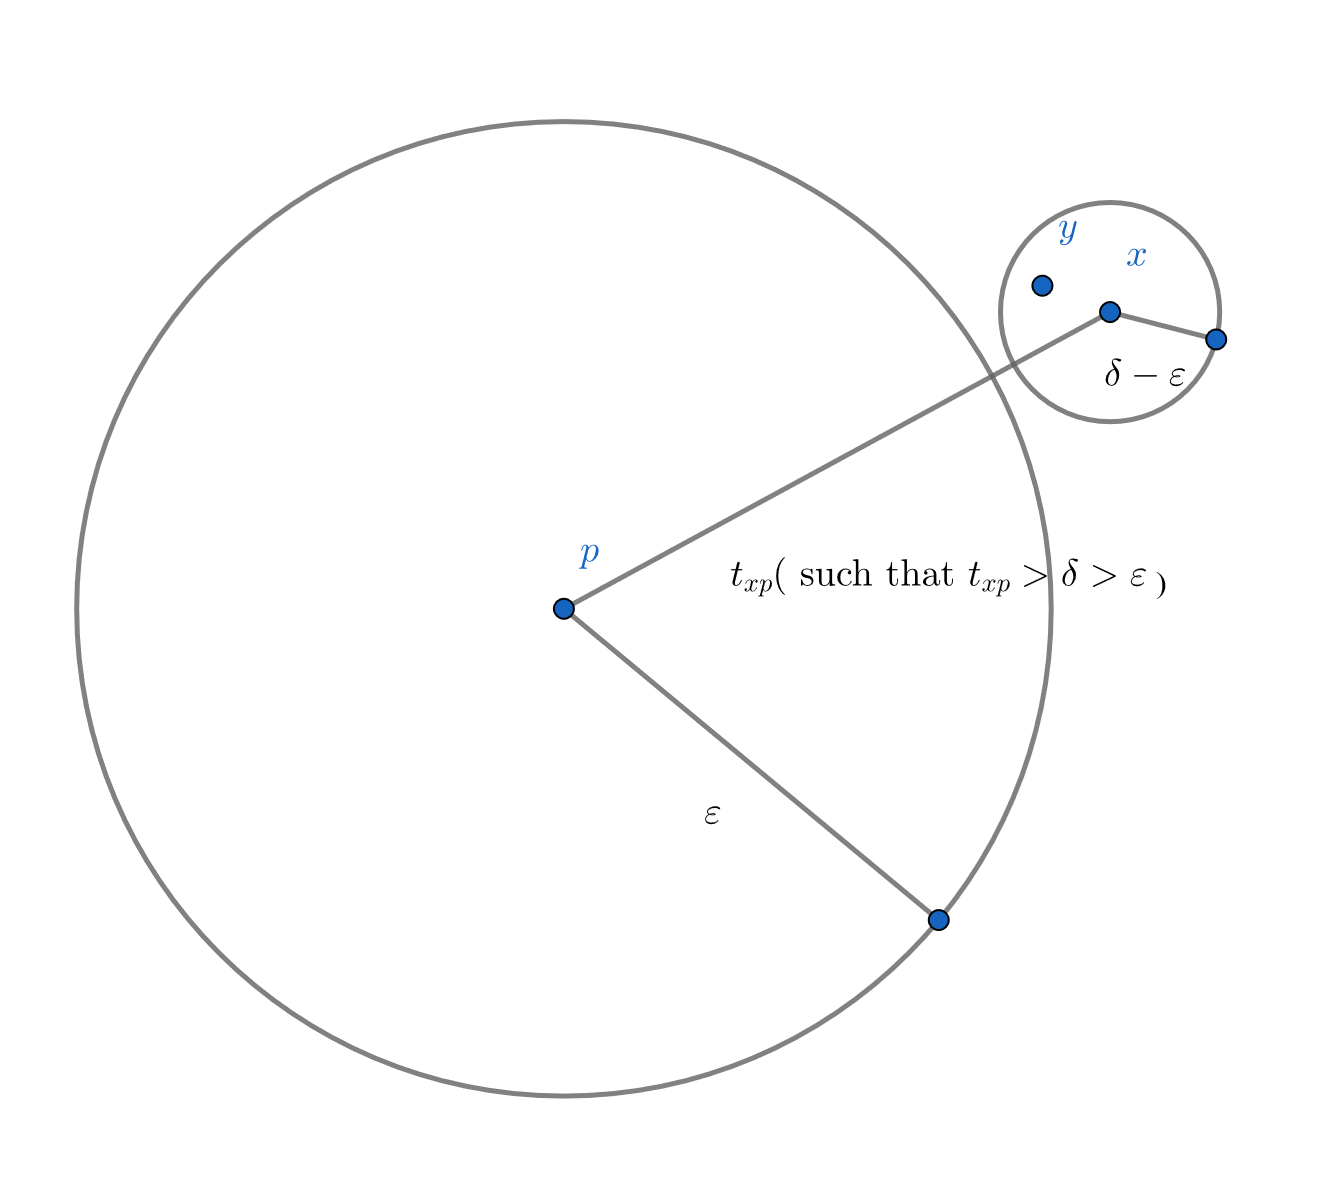
\includegraphics[width=0.5\linewidth]{Images/ballz.png}
    \caption{Figure for the proof: Closed balls are closed}
    \label{Closed balls are closed}
\end{figure}

\thmp{}{Compact sets are closed.}{\textbf{Method 1:}\\\\Let $E$ be compact. Consider a point $p \in E^c$. Let $\varepsilon_x$ be the "half" distance between a point $x \in E$ and $p$. Therefore, $B_{\varepsilon_x}(x)$ is completely outside $B_{\varepsilon_x}(p)$. Consider $\cup_{x \in E} B_{\varepsilon}(x) $ which is an open cover for $E$. This means there is a finite subcover 

$\{B_{\varepsilon_{x_1}}(x_1), B_{\varepsilon_{x_2}}(x_2), B_{\varepsilon_{x_3}}(x_3) \cdots, B_{\varepsilon_{x_k}}(x_k) \}$ such that $E \subset \cup_{i=1}^k B_{\varepsilon_{x_i}}(x_i)$. $B_{\varepsilon_{x_i}}(p)$ does not intersect with $B_{\varepsilon_{x_i}}(x_i)$. Therefore, $\cap_{i=1}^kB_{\varepsilon_{x_i}}(p)$ does not intersect with any $B_{\varepsilon_{x_i}}(x_i)$ for any $i$. Hence, it does not intersect with $\cup_{i=1}^k B_{\varepsilon_{x_i}}(x_i)$ which means $\cap_{i=1}^kB_{\varepsilon_{x_i}}(p)$ lies completely outside $E$. If we choose $\delta< min\{\varepsilon_{x_1},\varepsilon_{x_2} \cdots \varepsilon_{x_k}\}$, we would have $B_{\delta}(p) \subseteq \cap_{i=1}^kB_{\varepsilon_{x_i}}(p)$. This means that, for $p$ outside $E$, there would exist a $\delta$ such that the $\delta$-ball around $p$ is fully contained in $E^c$. This means that $E^c$ is open, hence, $E$ is closed.
\\\\ \textbf{Method 2:}\\\\ Consider $E$ to be compact, i.e, for every closed collection $\{F_{\alpha}\}$ such that $\cap_{\alpha} F_{\alpha} \subset E^c $, there exists a finite sub collection $\{F_{\alpha_1},F_{\alpha_2} \cdots F_{\alpha_k} \}$ such that $\cap_{j=1}^k F_{\alpha_j} \subset E^c$. Consider a point $p$ outside $E$, i.e, in $E^c$. Notice that $\cap_{\varepsilon \in \RR^+} B_{[\varepsilon]}(p)=\{ p\}$ which is in $E^c$. This would be a collection of closed sets whose intersection falls completely inside $E^c$. Hence, there would exist a finite subcollection such that $\cap_{j=1}^k B_{[\varepsilon_j]}(p)\subset E^c$ which means there would exist a neighbourhood around $p$ which is completely in $E^c$. Hence, $E^c$ is open, and $E$ is closed. 

}
\fact{$\phi$ and $X$ are both open and closed.}
\thmp{}{Closed subsets of compact sets are compact}{Consider $K \subset E$ where $E$ is compact and $K$ is closed. $K^C$ is, therefore, open. Consider an arbitrary open cover $\{F_{\alpha}\}$ for $K$. since $K\subseteq \cup_{\alpha} F_{\alpha}$, and $K^c$ is open, we have $X=\cup_{\alpha} F_{\alpha} \cup K^c$ which means $E \subset \cup_{\alpha}F_{\alpha} \cup K^c$. Since $E$ is compact, there would exist a finite subcover such that $E \subset \cup_{j=1}^n F_{\alpha_j} \cup K^c$. We then have $K \subset \cup_{j=1}^n F_{\alpha_j} \cup K^c$, which would mean $K \subset \cup_{j=1}^n F_{\alpha_j}$, whence, we see that $K$ is compact.}
\cor{If $F$ is closed, and $K$ is compact, then $F \cap K$ is compact}
\fact{A compact set is bounded}\pf{Consider (WLOG, a non empty compact set $E$) and an arbitrary point $q$ in $X$. $B_{\varepsilon}(x)$ for every $\varepsilon>0$ forms an open cover for $E$ (since it is basically $X$). Which means there is a finite subcover, i.e, a number $\varepsilon_0>0$ such that $E \subset B_{\varepsilon_0}(p)$ which makes $E$ bounded.}

\thmp{}{Finite union of compact sets is compact}{Let $K_1,K_2,\cdots K_r$ be $r$ compact sets. Let $K=\cup_{i=1}^rK_i$. Consider an open cover $F_{\alpha}$ whose union subsumes $K$. We have that, for every $i \leq r$, $K_i \subset \cup_{\alpha}F_{\alpha}$. Since each $K_i$ is compact, there exists a finite of $F_{\alpha}$ whose union subsumes $K_i$. For each $i=1,$ to $r$, we have a finite subcollection, therefore, taking the union of all these finite subcollections gives us a finite subcollection which subsumes whole of $K$. Hence $K$ is compact.

}
\rmkb{Note that finiteness in the above theorem is important. This is because, each compact may have finite subcollection, but at the end, the union of all these finite collections will be countable, not finite.}

\thmp{}{If $\{K_{\alpha} \}$ is a collection of compact sets such that for every finite subcollection $\{K_{\alpha_j}: 1\leq j\leq k\}$ we have that $\cap_{j=1}^k K_{\alpha_j} \neq \phi$. Then $\cap_{\alpha} K_{\alpha} \neq \phi$. In pithy words:\\\\\centering{{"If you have a collection of compact sets for which every finite subcollection's intersection is non-empty, the intersection of the whole collection is non empty"}{\\-\textit{Krishna, to Arjuna}}} }{Suppose, on the contrary, let $\cap_{\alpha} K_{\alpha}=\phi$ which means $\cup_{\alpha} K^c_{\alpha}=X$ which means for every for some $\alpha_0$, we have $K_{\alpha_0} \subset \cup_{\alpha} K^c_{\alpha}$, where $\cup_{\alpha} K^c_{\alpha}$ is an open cover of $K_{\alpha_0}$. This implies that there exists a finite subcollection $\{K^C_{\alpha_1},K^C_{\alpha_2} \cdots K^C_{\alpha_r}\}$ such that $K_{\alpha_0}\subset \cup_{j=1}^r K^C_{\alpha_j} \implies \cap_{j=1}^r K_{\alpha_j} \subset K^C_{\alpha_0}$. But this means $\cap_{j=1}^r K_{\alpha_j} \cap K{\alpha_0}=\phi$, which is absurd since all finite intersection is non empty.

}
\cor{If $K_1,K_2,\cdots$ is a sequence of non-empty compact sets such that $\cdots K_n \subset K_{n-1} \cdots K_3 \subset K_2 \subset K_1$, then $\cap_{i=1}^{\infty} K_i$ is non empty.

}
\thmp{Compactness $\implies$ Limit point Compact}{If $K$ is a compact set and $E$ is an infinite subset of $K$, then $E$ has a limit point in $K$}{Suppose that $E$ has no limit point in $K$. Since $K$ is closed, $E$ must have no limit points. Hence, $E$ is closed. Since closed subsets of compact sets are compact, $E$ is compact. If no point of $E$ is a limit point of $E$, then $\forall x \in E$, $\exists \varepsilon_x>0$ such that no point of $E$ apart form $x$ itself falls into the $\varepsilon_x$-ball of $x$. Consider the open cover $\{B_{\varepsilon_x}(x): x\in E\}$ of $E$. This has a finite subcover $\{B_{\varepsilon_{x_1}}(x_1), B_{\varepsilon_{x_2}}(x_2), \cdots B_{\varepsilon_{x_l}}(x_l)\}$. We see that $E \subseteq \cup_{j=1}^l B_{\varepsilon_{x_j}}(x_j)$. But since for every $\varepsilon_{x_j}$-ball around $x_j$, no point in $E$ except $x_j$ resides, $\cup_{j=1}^lB_{\varepsilon_{x_j}}(x_j)$ will have utmost finite points. Since an infinite set $E$ cannot be the subset of a finite set, we have a contradiction. }

\defn{k-cell}{a $k$-cell, $E$ is a set in $\RR^k$ such that $E:=\{\vec{x}=(x_1,x_2,\cdots,x_k) \in \RR^n: a_j\leq x_j \leq b_j \text{ for given }a_j \text{ and } b_j \text{ for every } 1\leq j\leq k  \}$\\\\ A $k$-cell is basically a $k$ dimensional cuboid.  }

\thmp{}{$k$-cells are closed}{Consider a $k$-cell $E$. Consider a point $z$ not in $E$, i.e, $\exists j_0$ such that either $z_j<a_j$ or $z_j>b_j$. WLOG, take the case of $z_j<a_j$. Let $0<\delta<(a_j-z_j)$. Consider a point $q$ in the $\delta$-ball around $z$. i.e, $d(z,q)<\delta \implies \sqrt{(z_1-q_1)^2+(z_2-q_2)^2+\cdots+(z_k-q_k)^2}<\delta \implies (z_1-q_1)^2+(z_2-q_2)^2+\cdots+(z_k-q_k)^2 <\delta^2<(a_j-z_j)^2 \implies 0<(q_j-z_j)^2<(a_j-z_j)^2$ $\implies q_j<a_j$. Hence $q \not\in E$, which implies there exists, for every $x$ in $E^c$, a $\delta$ for which the $\delta$-ball around $x$ is fully contained in $E^c$ which means $E^c$ is open. This implies $E$ is closed. Same argument applies for the case where $z_j>b_j$.}

\thmp{}{Closed intervals in $\RR$ are compact}{Let $\II$ be, WLOG, $[-a,a]$. Suppose it is not compact. i.e, There is an open cover $G_{\alpha}$ of $\II$ such that there exists no finite subcover. $\forall x \in \II$, $\exists \alpha_x$ such that $x \in G_{\alpha_x}$ and $\exists \varepsilon_x$ such that $B_{\varepsilon_x}(x) \subset G_{\alpha_x}$. $\cup_{x} B_{\varepsilon_x}(x)\subset \cup_{\alpha} G_{\alpha}$ is an open cover for $\II$. note that, if no finite subcover for $G_{\alpha}$ exists, then no finite subcover for $B_{\varepsilon_x}(x)$ exists either. So we can safely work with $B_{\varepsilon_x}(x)$. Split the interval into two halves, $[-a,0]$ and $[0,a]$. One of these intervals is not finitely covered by $B_{\varepsilon_x}(x)$, for if not, the whole thing would be finitely covered. let that interval which is not finitely covered be $\II_1$. This interval's size is $a$. Split this interval into two again. Yet again, one of the halves must not be finitely covered, for if not, $\II_1$ would be finitely covered, which is contradictory. Let this interval be $\II_2$. This is of size $\frac{a}{2}$. Yet again, keep doing this process to obtain a sequence of intervals $\II_j$, sized $\frac{a}{j}$, which are not finitely covered. These are nested intervals, non empty, and closed. From nested intervals theorem, we see that a point $\xi$ exists in $\cap_{j=1}^{\infty}\II_j$. $\xi$ is a point in $\II$, and there is a corresponding $\varepsilon_{\xi}$. Consider that $j_0$ for which $\frac{a}{j_0}<\frac{\varepsilon_{\xi}}{2}$. We know from Archimedean such a $j_0$ exists. This means that the interval $\II_{j_0}$ containing $\xi$, sized $\frac{a}{j_0}$, is completely inside the $\varepsilon_{\xi}$-ball around $\xi$, which means it is finitely covered. Contradiction. Hence, $\II$ is compact.}
\cor{Since intervals of the form $[-a,a]$ are compact, every closed interval of the form $[a,b]$ is compact since it would be a closed subset of an interval of the form $[-x,x]$.}
Generalisation:
\thmp{}{$n$-cells are compact}{Consider $K:=\{ \vec x \in \RR^n: -a \leq x_j \leq a; \forall j \leq n\}$ to be non-compact. There is an open cover $G_{\alpha}$ of $K$ such that there exists no finite subcover. $\forall x \in K$, $\exists \alpha_x$ such that $x \in G_{\alpha_x}$ and $\exists \varepsilon_x$ such that $B_{\varepsilon_x}(x) \subset G_{\alpha_x}$. $\cup_{x} B_{\varepsilon_x}(x)\subset \cup_{\alpha} G_{\alpha}$ is an open cover for $K$. note that, if no finite subcover for $G_{\alpha}$ exists, then no finite subcover for $B_{\varepsilon_x}(x)$ exists either. So we can safely work with $B_{\varepsilon_x}(x)$. Till here, everything is the same as the $1$-d case. Note that here, the $n$-cell is constructed by taking the cartesian product of $n$- intervals in $\RR$ of the kind $[-a,a]$. Construct $2^n$ subdivisions of $K$ by halving each interval $[-a,a]$ in the construction of $K$. The total number of subdivisions we make would be $2 \times 2 \times \cdots \times 2$, n times (simple combinatorial argument: for each $i$, there exists $2$ choices, the two half intervals, for crossing. From $i=1$, you have 2 choices, likewise, $j=2,3,\cdots n$). We assume that atleast one of these $2^n$ subdivisions are not finitely covered by $\{ B_{\varepsilon_x}(x) \}$. We let this one be $K_1$, whose each interval size is now $a$. Subdivide this yet again into $2^n$ subsets, and assert that one of these subdivisions is not finitely covered. Call this $K_2$, whose each interval is of size $\frac{a}{2}$. Construct a sequence of sets $K_j$, each of whose intervals are sized $\frac{a}{j}$. Each $K_j$ is closed and non empty, hence compact, and are nested. Therefore, $\cap_{j=1}^{\infty} K_j \neq \phi$. Let $p \in \cap_{j=1}^{\infty} K_j$. For this $p$, there would exist a $\varepsilon_p$ and the corresponding ball $B_{\varepsilon_p}(p)$. We require one of our $K_j$ $n$-cell to fall into this $\varepsilon_p$ ball. Let $\delta$ be smaller than $\frac{\varepsilon_p}{2}$. Let $p$ be the centre of the $\delta-$ball. Let $p$ be the centre of the $n$-cube $H$ in the following construction: Consider $w$ to be the side length of $H$. We require the diagonal length $w\sqrt{n}=\delta$, which gives us $w=\frac{\delta}{\sqrt{n}}$. Consider $H$ such that each side is the interval $[p_j-\frac{w}{2},p_j+\frac{w}{2}]$. This would force $p$ to fall in the centre of the $n$-cube $H$. This cube is fully contained in the $\delta$ ball of $p$ which is contained in the $\varepsilon_p$ ball of $p$. We consider that $n$ cell $K_j$ for which each side $\frac{a}{j}<w$. This can be found, and hence, the this $K_j$ cell is finitely covered by $B_{\varepsilon_p}(p)$, which is absurd. Hence, $K$ is compact.}

\begin{figure}[h]
    \centering
    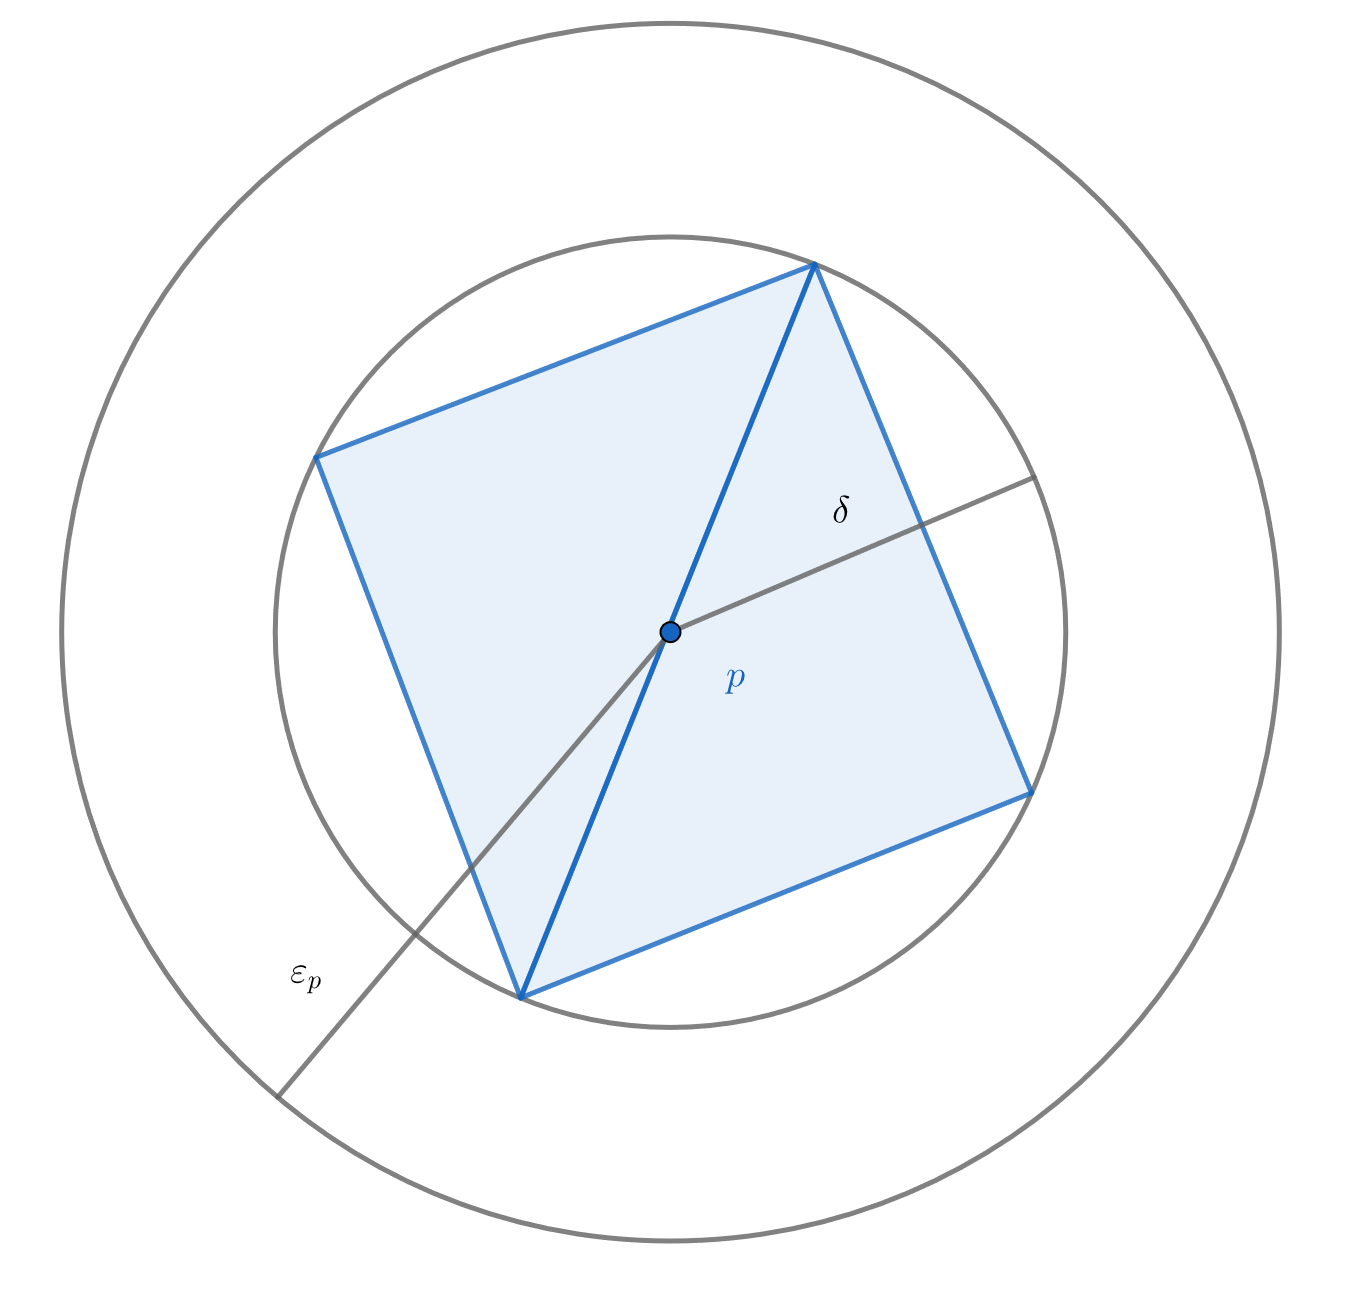
\includegraphics[width=0.5\linewidth]{Images/kcellz.png}
    \caption{Figure for the proof: $n$-cells are compact.(The $\varepsilon_p$-ball around $p$, and the $n$-cell construction)}
    \label{fig:ncellz}
\end{figure}

\rmkb{We proved the result for $k$-cells of the kind $[-a,a]^k$, but it is easily generalised by noting that arbitrary $k$-cells are contained in some $k$-cell of the above kind. By virtue of being closed, they also are compact.}
\thmp{Heine-Borel}{Given a set $E \subset \RR^n$, the following are equivalent:
\begin{enumerate}
    \item $E$ is closed and bounded
    \item $E$ is compact
\end{enumerate}}{$\impliedby$) We know that all compact sets are closed.\\\\
$\implies$) If $E \subset \RR^n$ is closed and bounded, it is contained in some $n$-cell, which is compact. By virtue of being a closed subset of a compact set, $E$ is also compact.}
\thmp{}{If $\{ x_n\}$ is a sequence in $X$ convergent to $x\in X$, then the set $\{x_n\}$ has only one limit point, which is $x$.}{That $x$ is a limit point is clear. We note that $\forall \varepsilon>0$, $\exists n_0$ such that $\forall n \in \NN, n\geq n_0$ we have $d(x_n,x)<\varepsilon$. i.e, beyond a particular $n_0$, every point of $\{X_n\}$ falls in the $\varepsilon$-ball of $x$. Therefore, only finite points lie outside this $\varepsilon$-ball of $x$. Suppose it has another limit point $y$, other than $x$. Therefore, there would exist a $\delta$ such that the $\delta$-ball around $y$ lies completely outside the $\delta$-ball around $x$. This means that, only finite points of $x_n$ lie in the $\delta$ ball of $y$, making it unviable to be a limit point.}

Extending Heine Borel we have:
\thmp{(Extension)}{For a subset $E \subset \RR^n$, the following are equivalent: 
\begin{enumerate}
    \item $E$ is closed and bounded
    \item $E$ is compact
    \item every infinite subset $K$ of $E$ has a limit point in $E$
\end{enumerate}}{$(1)\implies(2)$) Heine Borel\\\\
$(2)\implies(3)$) Already seen\\\\
$(3)\implies(1)$) Let us assume that $E$ is either not closed, or not bounded. We start by assuming it is not closed. Which means that $\exists q$ outside $E$ such that there exists a sequence in $E$ that converges to $q$. We take this sequence $\{x_n\}$ as our infinite set, and we see that, from the previous theorem, this has only one limit point $q$, which lies outside $E$. Hence, there exists an infinite set $\{x_n\}$ which has no limit point in $E$. 
\\\\ Suppose that $E$ is unbounded. We then have that, $\forall x \in X$, $\forall \varepsilon>0$, $\exists y \in E$ such that $d(x,y)> \varepsilon$. Fix some $x_0$ in $X$. Choose some $y_0$ that is a distance $z_{00}=d(y_0,x_0)$ away from $x_0$. Look if there is a point $y_1$ so that its distance from $x_0$ is more than $z_{00}$ but less than $2(z_{00})$. If it doesn't exist, check for less than $3(z_{00})$. Find some $k_1(z_{00})$ so that distance of $y_1$ to $x_0$ is more than $z_{00}$ but less than $k_1(z_{00})$. Same way, for $y_2$, find $y_2$ so that its distance from $x_0$ is more than $k_1{(z_{00})}$ but less than some other $k_2(z_{00})$. Inductively, find $y_j$ whose distance is more than $k_{j-1}(z_{00})$ but less than $k_j(z_{00})$. Note that $1<k_1<k_2<\cdots$. Hence, for any $\varepsilon$-ball around $x_0$, only finite $y_j$ exists in that ball, since there would exist some $k_{q}(z_{00})$ and $k_{q-1}(z_{00})$ between which $\varepsilon$ lies. And inside $k_{q-1}(z_{00})$ ball around $x_0$, utmost finite points $y_j$ exists. Hence, $x_0$ is clearly not a limit point for the set of $y_j$-s. Consider any other point $a \in X$. For some every $\varepsilon$-ball around $x_0$, only finite points exists. For some, perhaps larger $\delta$-ball around $a$, a chosen $\varepsilon$-ball around $x_0$ gets subsumed into the $\delta$-ball around $a$. This implies that only finite points of $y_j$-s exists in the $\delta$-ball around $a$ as well, making $a$ a non viable limit point. We see that, for this infinite subset $\{y_j\}$ of $E$, no limit point exists.  }
\begin{figure}[h]
    \centering
    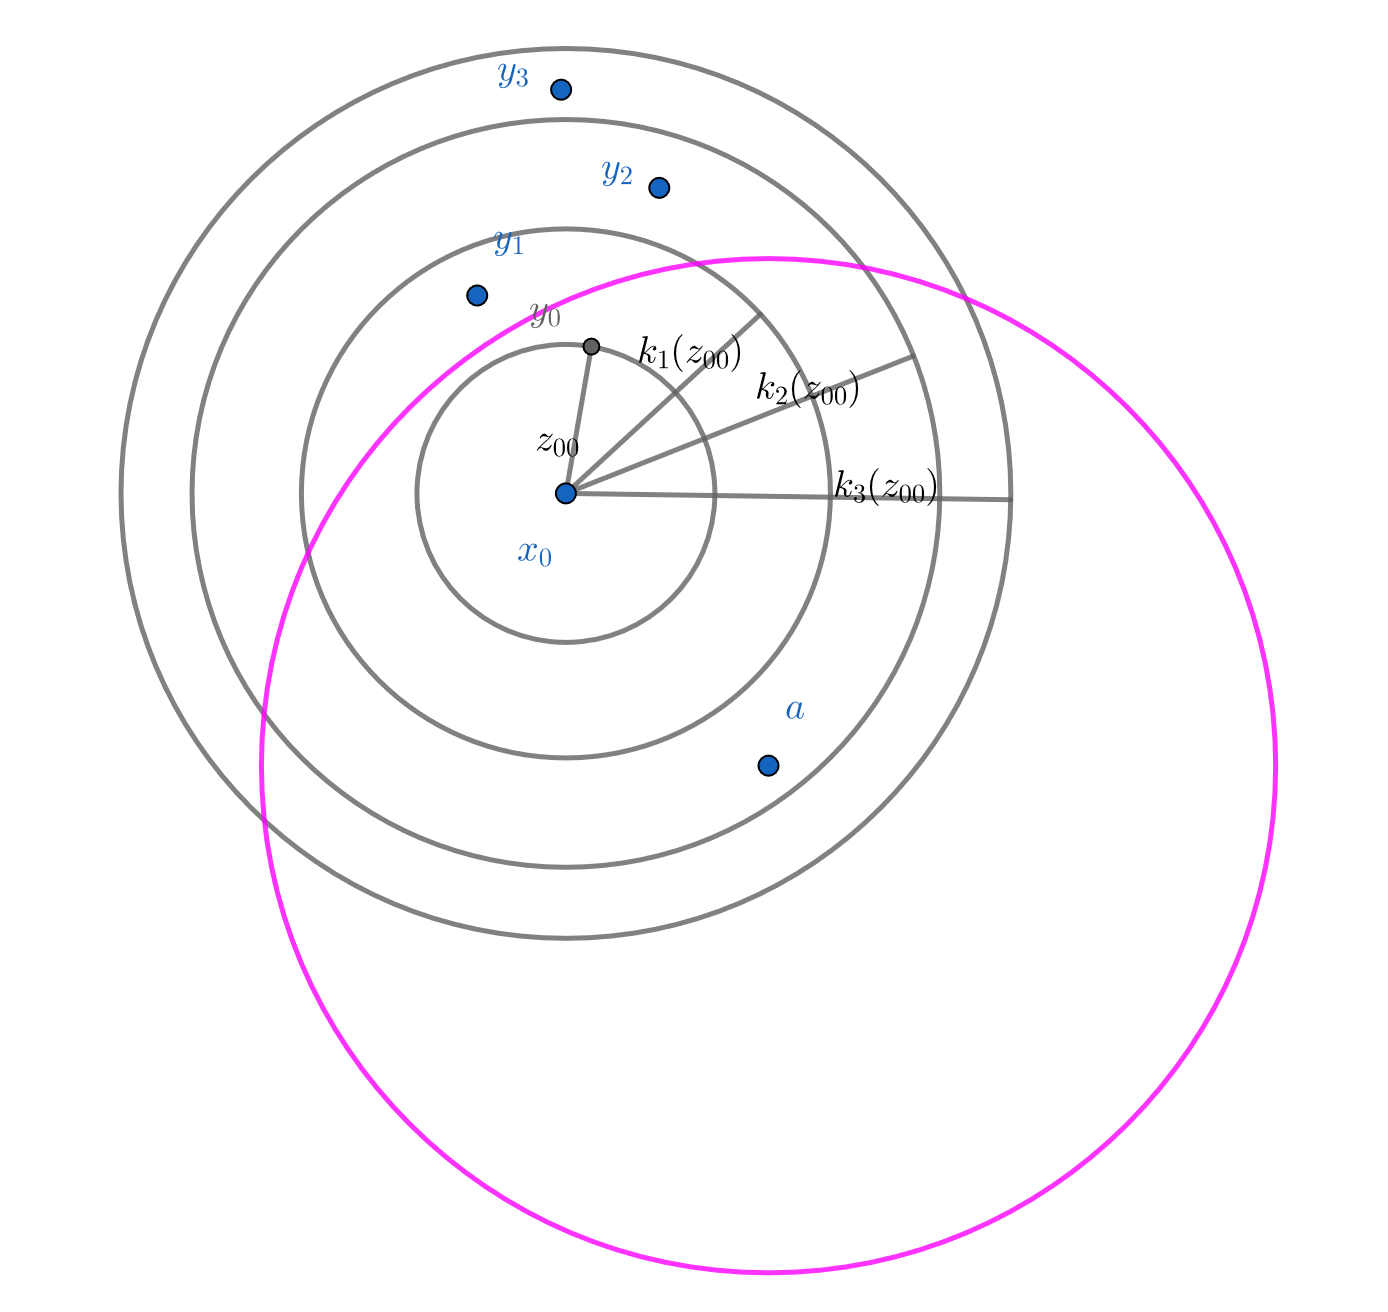
\includegraphics[width=0.5\linewidth]{Images/limptcompact.png}
    \caption{Figure for proof: Lim point compact $\implies$ closed+bounded. (The construction of an unbounded sequence)}
    \label{fig:lptcpt}
\end{figure}
\rmkb{In the previous proof, we note that (3), which is called Limit Point Compactness, implies (1) Closed and Bounded, in any metric space, not just $\RR^n$, as we see in the proof, no property of $\RR^n$ was used.\\\\
\textbf{Spoiler Alert:} In any metric space, Limit Point Compact $\iff$ Compact }

\thmp{Weierstrass Theorem}{Every Bounded, infinite set in $\RR^n$ has a limit point in $\RR^n$.}{If a set is bounded in $\RR^n$, it is the subset of a compact set (i.e, a closed and bounded set). From the previous equivalence, an infinite subset $E$ of a compact set has a limit point in the compact set, which means the bounded, infinite set we have has a limit point in the compact set that contains it, hence, it has a limit point in $\RR^n$.}
\rmkb{The above "Weierstrass Theorem" is just the "Bolzano-Weierstrass" Theorem we saw in sequences. Actually, the "Bolzano-Weierstrass" Theorem is a direct corollary of the more general "Weierstrass Theorem". Let $\{x_n\}$ be any sequence in $\RR$ that is bounded. This means that this sequence is the subset of a compact set, hence, has a limit point in $\RR$. This implies, a subsequence of $\{x_n\}$ converges in $\RR$. Hence, every bounded sequence has a convergent subsequence. }

\fact{Let $X=\RR^n$. The closure of any open ball is the corresponding closed ball.}
\pf{Consider $B:=B_{\delta}(x_0):=\{y \in \RR^n: ||y-x_0||<\delta \}$. Let $z_0$ be a point on the rim of $B$, i.e $d(x_0,z_0)=\delta$. Such a point obviously exists. Consider $\vec\gamma(t)=t\vec z_0 +(1-t)\vec x_0$ with $t \in(0,1)$.
For every $t \in(0,1)$, $\vec \gamma(t)$ belongs in $B$. To see this, consider $||\vec\gamma(t)-\vec x_0||=||t\vec z_0+(1-t)\vec x_0-\vec x_0||=||t(\vec z_0- \vec x_0) ||=t||\vec z_0-\vec x_0||<t(\delta)<\delta$. Suppose we are given an arbitrary $\eta>0$. Does there exist a $t \in(0,1)$ so that $\vec \gamma(t)$ belongs in the $\eta$-ball of $\vec z_0$? i.e, we need a $t$ so that $||\vec \gamma(t)-\vec z_0||=||t\vec z_0+(1-t)\vec x_0 -\vec z_0||=||(1-t)(\vec z_0-\vec x_0)||<\eta$ $\implies (1-t)||\vec z_0 -\vec x_0||<\eta \implies 1-t< \frac{\eta}{\delta} \implies 1-\frac{\eta}{\delta}<t<1$. Such a $t$ exists for every $\eta$. Hence, $\vec z_0$ is a limit point of $B$ (by virtue of there existing a sequence of $\vec \gamma(t_j)$ that converges to $\vec z_0$).
Hence, every point on the rim is a limit point. Moreover, no point $w$ so that $d(w,x_0)>\delta$ is a limit point of $B$, since there would exist an $\varepsilon$-ball around $w$ so that no point of $B$ falls into it (from openness). Hence, closure of $B$ is the corresponding closed ball, in $\RR^n$.

}
\section{Perfect Sets}
\defn{Perfect Set}{A set $E \subset X$ is perfect if every point of $E$ is a limit point of $E$, and $E$ is closed}
\thmp{}{Perfect subsets in $\RR^n$ are uncountable.}{Suppose $E$ is a perfect set in $\RR^n$ but is countable. i.e, it can be enumerated as $E=\{x_1,x_2,\cdots \}$.
\\\\ Choose $x_1$, and $\varepsilon_0=1$. Let $V_0$ denote the $\varepsilon_0$-ball around $x_1$. This ball is non empty, moreover, $\bar{V_0} \cap E$(which is the corresponding closed ball of $V_0$) is non empty, and is compact by virtue of being closed and bounded. Inside, $V_0 \cap E$, there exists infinite points of $E$, since $x_1$ is a limit point of $E$.
\\\\ Choose an arbitrary point $z_1$ in $V_0$ that is not $x_1$. Now let $\varepsilon_1<d(x_1,z_1)$. Let $V_1$ be the $\varepsilon_1$-ball around $z_1$. Notice the following: $z_1$ is a limit point of $E$, hence, there are infinite points of $E$ in $V_1$. $x_1$ is not in $\bar{V_1}$. $\bar{V_1}\cap E$ is closed, bounded and non empty, hence Compact. 
\\\\ Choose a point $z_2$ in $V_1$ that is not $x_2$, and let $\varepsilon_2<min\{\varepsilon_1, d(x_2,z_2)\}$. Let $V_2$ be the $\varepsilon_2$-ball around $z_2$. Note that, $x_2$ is not in $\bar{V_2}$. Also note yet again that there are infinitely many points of $E$ in $V_2$. It is crucial to note now that $\bar{V_2}\cap E \subset \bar{V_1}\cap E\subset \bar{V_0} \cap E$.
\\\\Suppose you have already constructed $V_k$ by finding $z_k$ in $V_{k-1}$ that is not $x_k$ and an $\varepsilon_k<min{d(z_k,x_k),\varepsilon_{k-1}}$ such that $x_k \not\in \bar{V_k}$, $\bar{V_k}\cap E$ is compact, non empty and $\bar{V_k}\cap E \subset \bar{V_{k-1}}\cap E \cdots$.
\\\\Now, choose $z_{k+1} \neq x_{k+1}$, inside $V_k$. Choose $\varepsilon_{k+1}<min\{d(z_{k+1},x_{k+1}),\varepsilon_k\}$. Let $V_{k+1}$ be the $\varepsilon_{k+1}$-ball around $z_{k+1}$. Yet again, we see that $\bar{V_{k+1}} \cap E$ is non empty, $x_{k+1}$ is not in $\bar{V_{k+1}}$, and $\bar{V_{k+1}}\cap E \subset \bar{V_{k}}\cap E$. Hence, we have a sequence of non empty, nested compact sets. This implies that $\exists \xi \in E \subset \RR^n$ such that $\xi \in \cap_{i=1}^{\infty} (\bar{V_i}\cap E)$. Is $\xi$ any one of $x_j$ enumerated? No, because if it was, from the construction, $x_j$ would not belong in $V_j$. Hence, $\xi$ is not in the enumeration of $E$. Contradiction.}
\begin{figure}[h]
    \centering
    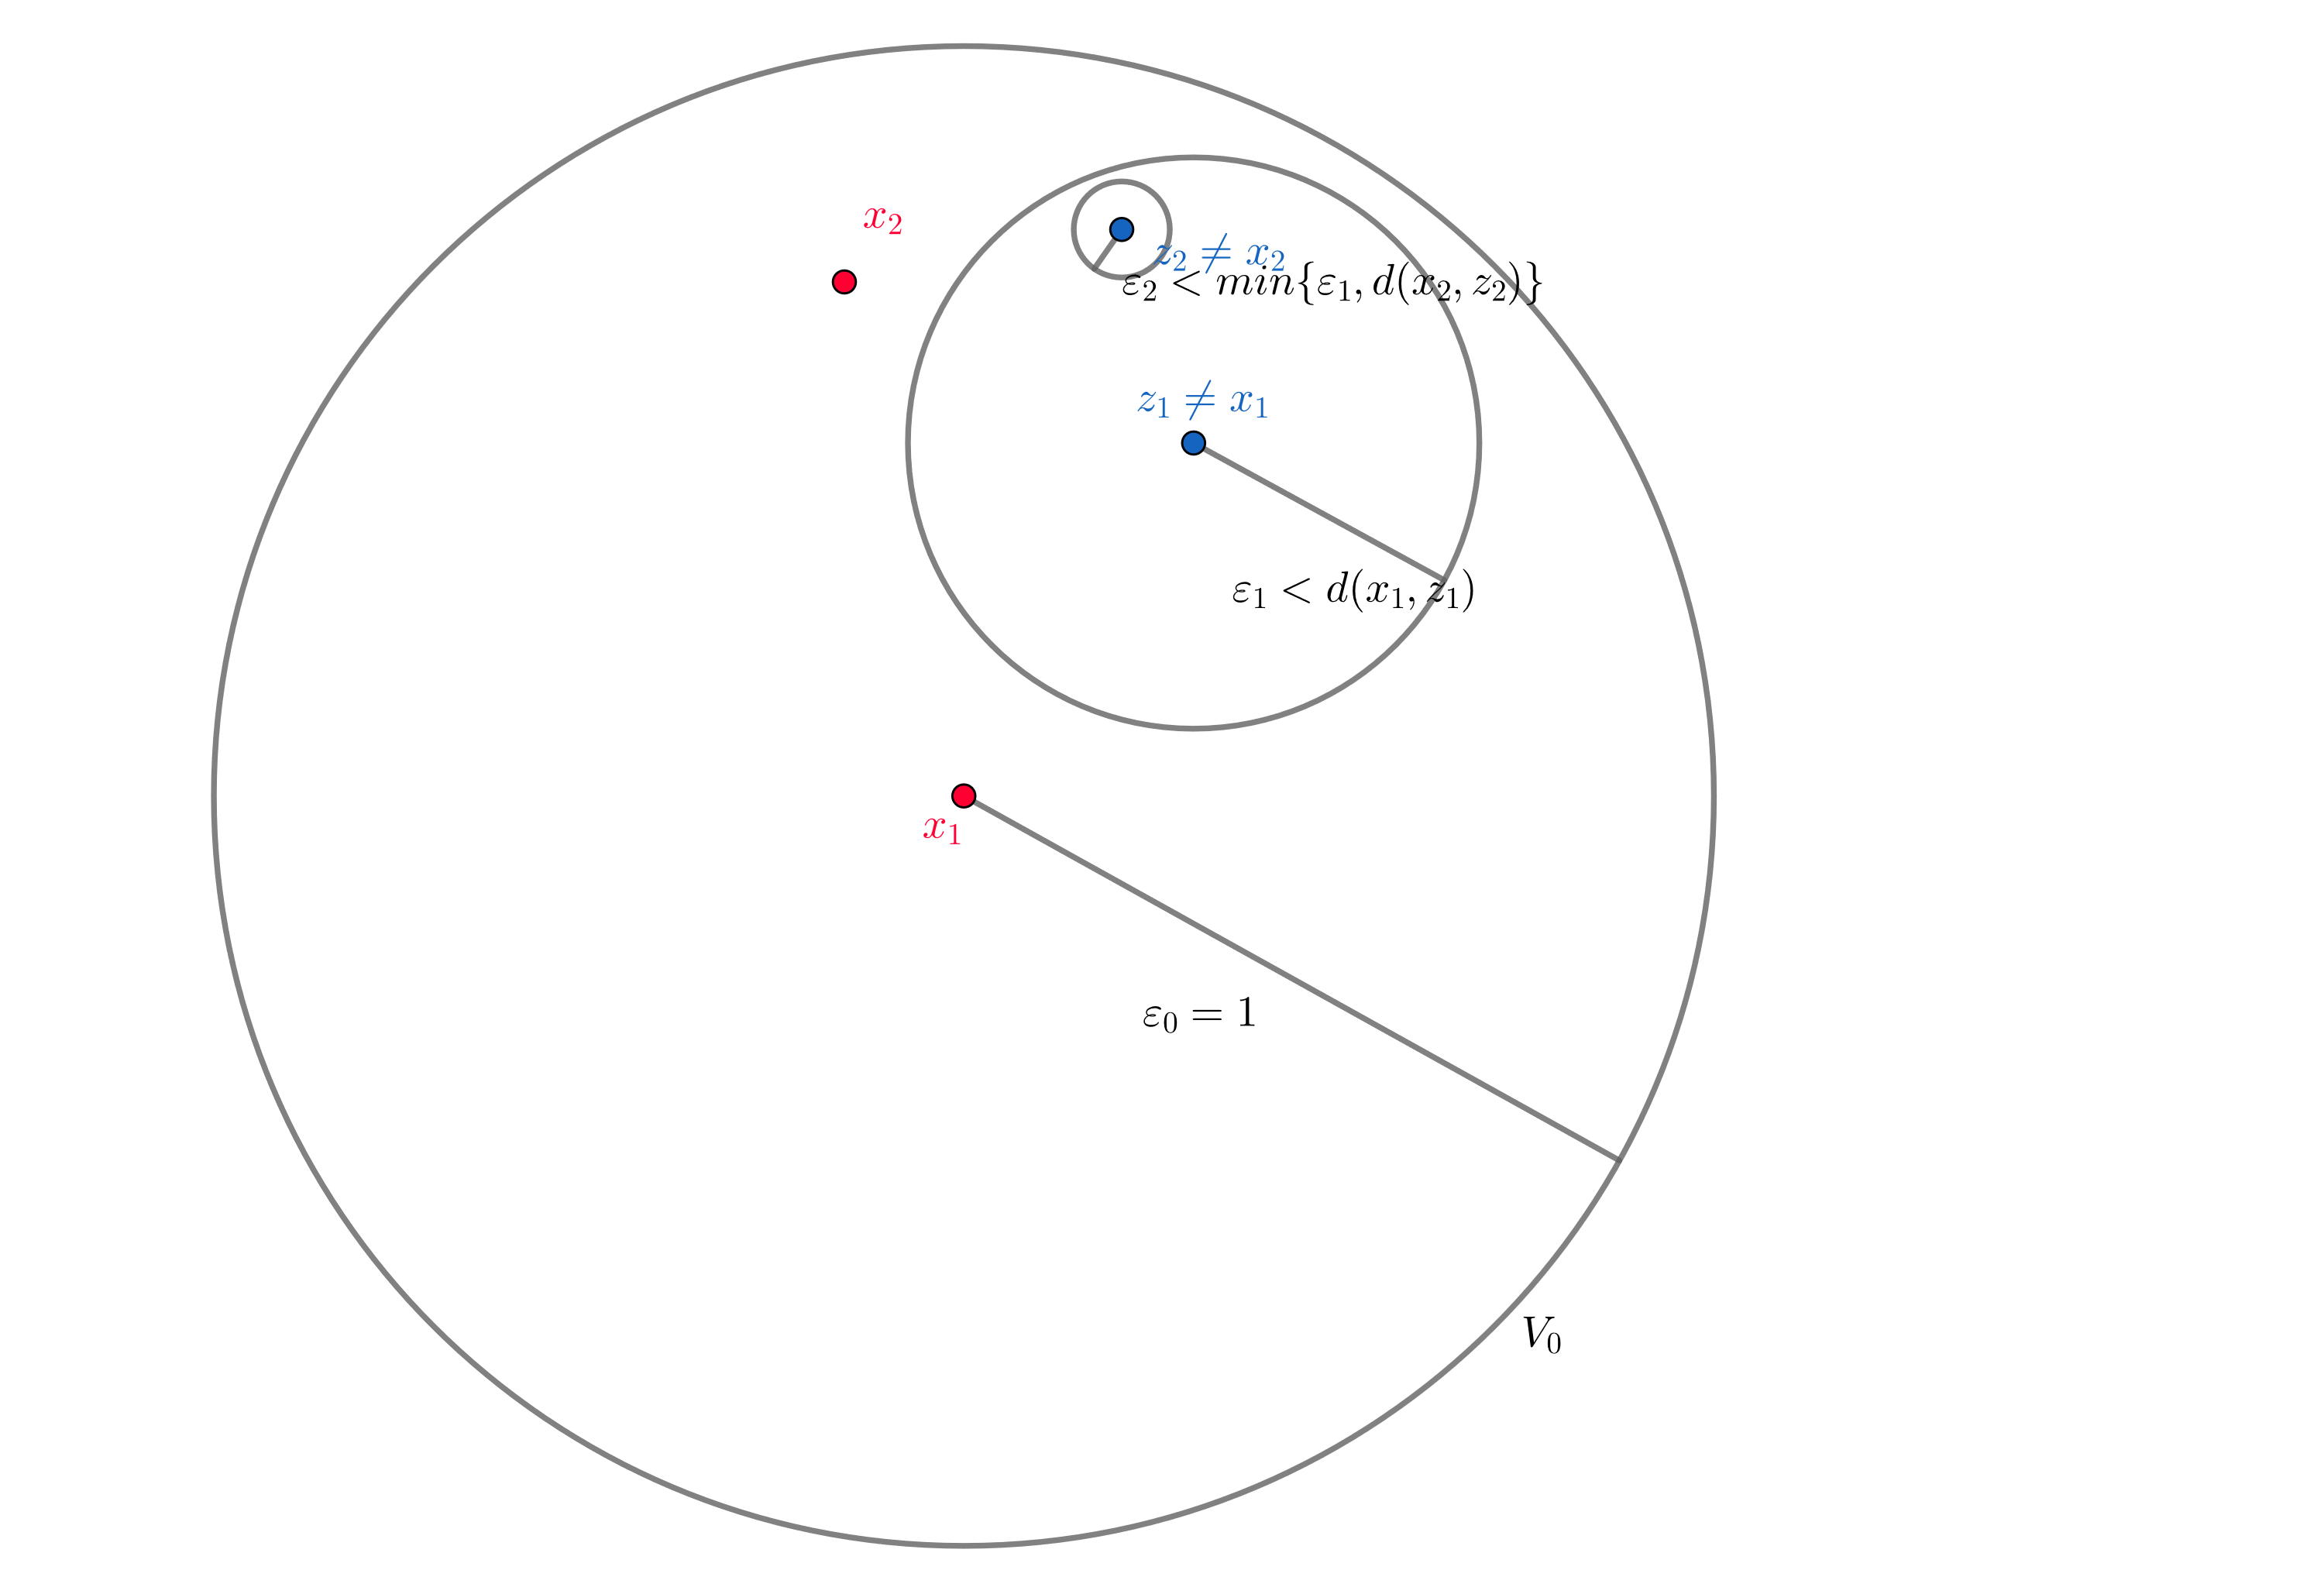
\includegraphics[width=1.0\linewidth]{Images/perfectsetz.png}
    \caption{Figure: Perfect sets are uncountable. Construction of the nested sequence of compact sets by choosing $z_k\neq x_k \in V_{k-1}$.}
    \label{fig:perfectunctbl}
\end{figure}
\newpage
\rmkb{It is easily seen that, closed intervals in $\RR$ are perfect: From density theorem, for every point in $I$, there would exist a sequence of rationals converging to that point. Moreover, closed intervals in $\RR$ are closed since closed balls in metric spaces are closed. Therefore, we see that intervals are uncountable.}
\subsection{The Cantor Set}
The following is the construction of an uncountable, perfect set that contains no intervals: The Cantor Set.
\\\\ Let $I_0=[0,1]$. size of the interval(s) in $I_0$ is $1$, and there are $2^0=1$ intervals.
\\\\ Let $I_1=[0,\frac{1}{3}]\cup[\frac{2}{3},1]$ be constructed by trisecting $I_0$ and tossing the middle one. Here, we have each interval sized $\frac{1}{3^1}$, and there are $2^1=2$ intervals total.
\\\\Let $I_2=[0,\frac{1}{9}]\cup[\frac{2}{9},\frac{3}{9}]\cup[\frac{6}{9},\frac{7}{9}]\cup[\frac{8}{9},1]$ be generated by taking each of the two sub intervals in $I_1$, trisecting them, and tossing the middle one, and joining them finally. We have each interval sized $\frac{1}{3^2}$ and there are $2^2=4$ intervals total.
\\\\Inductively keep making these trisections+tossings to make a sequence of closed, nested intervals (Compact, too) $I_k$, each containing $2^k$ intervals each of size $\frac{1}{3^k}$.
\\\\ Finally, define the Cantor set $P$ as $$P:= \big.\cap_{i=1}^{\infty}I_i $$ Note that $P$ is compact since it is the closed subset of a compact set. It is also non empty by virtue of being the intersection of a sequence of nested, non empty, compact sets.
\\\\Note that, no interval of the kind $[a,b]$ exists in the Cantor Set. The size of each interval in $I_j$ is $\frac{1}{3^j}$. We can find $j$ so that $\frac{1}{3^j}<b-a \implies \frac{1}{b-a}<3^j \implies \log_{3}(\frac{1}{b-a})<j$. For such $I_j$, we notice that $[a,b]$ has "inbetween" points that doesn't exist in any of $I_j$'s intervals. Hence, taking the intersection, these "inbetween" terms don't survive. Hence, no intervals exist.
\thmp{}{The Cantor set $P$ is perfect.}{We already know that the Cantor set is closed. We need to show that every point in the cantor set is a limit point. First, observe that, for any $I_k$, if $z$ is the end point of any of the sub interval of $I_k$, it survives the $\infty$-intersection. This is because, after $I_k$-s trisection, the end points still stay endpoints. Let $\xi$ be any point in the cantor set, which means it is a point in every $I_k$. Let $\delta>0$ be given. Consider the interval $(\xi-\delta,\xi+\delta)$. This interval is sized $2\delta$. $\xi$ exists in one of the sub intervals of $I_k$ for all $K \geq k_0$ for some $k_0$. Choose $j$ so that $\frac{1}{3^j}<\delta$. Then, the interval in $I_j$ containing $\xi$ would fall completely inside $(\xi-\delta,\xi+\delta)$. Choose $q$ as one of the end points of this sub interval of $I_j$. Therefore, $\forall \xi \in P$, $\forall \delta>0$, $\exists q \in P, q \neq \xi$ so that $q\in (\xi-\delta,\xi+\delta)$. Therefore, every $\xi \in P$ is a limit point of $P$. Hence, $P$ is perfect.}

\subsection{Connected Sets}
\defn{Separated Sets}{$A \subset X$ and $B \subset X$ are said to be \emph{separated} if $\bar{A} \cap B=
\bar{B}\cap A=\phi$, i.e, they are disjoint and no point of one, is the limit point of the other.}
\defn{Connected Set}{A set $E\subset X$ is said to be \emph{connected} if it is \emph{not} the union of two non-empty separated sets.
In other words, for every "split" of $E$ into two non empty sets, none of them are separated. Even if one split of $E$ is separated, then $E$ is \emph{not connected}.}
\exm{Separated $\implies$ Disjoint, but Disjoint $\not\implies$ Separated.}{$[0,1]$and $(1,2)$ are disjoint, but are not connected since a sequence in $(1,2)$ converges to $1$ in $[0,1]$.}
\thmp{}{$E \subset \RR$ is connected $\iff$ $\forall x,y \in E$, $x<z<y \implies z\in E$.}{$\implies$)
Suppose $\exists x_0,y_0 \in E$ so that $\exists z, x_0<z<y_0$, but $z \not\in E$. Consider $A:=(-\infty,z)$ and $B:=(z,\infty)$.
$A$ and $B$ are seen to be separated, and $E$ is a subset of $A \cup B$, which makes it disconnected.
\\\\ $\impliedby)$ Suppose that we have $E$ disconnected, which means it is the union of two 
separated sets $A$ and $B$ that are non-empty. $x_0 \in A$ and $y_0 \in B$. Consider $z(t)=x_0+t(y_0-x_0)$ for $t\in [0,1]$.
Note that $z(0)=x_0$ and $z(1)=y_0$.
\\\\ Conjecture: There exists a $t_B \in (0,1)$ so that for every $t<t_B$, $z(t)$ does not belong in $B$. If it is not true,
then for every $t \in (0,1)$, there exists a point $t_B<t$ so that $z(t_B)$ is in B. Choose $t=1$ to get $z(t_1)$ in $B$.
Chooe $t=\frac{t_1}{2}$ to get $z(t_2)$ in $B$ with $t_2<t_1$ and $t_2<\frac{1}{2}$. Keep going with $t=\frac{t_{n-1}}{2^{n-1}}$ to get $z(t_n)$ in $B$ with $t_n<t_{n-1}$ and $t_n<\frac{1}{2^{n-1}}$. 
This gives us a sequence $z(t_k)$ which we can see is monotone decreasing assuming $x_0<y_0$. This sequence converges to $z(0)$ which is in $A$ which means that there exists a sequence in $B$, $z(t_n)$ that converges to $A$. Absurd.
\\\\ In a similar vein, we can show that there exists $t_A \in (0,1)$ so that for every $t>t_A$, $z(t)$ is not in $A$. 
Consider $$S_A:=\{ t \in [0,1]: z(t)\in A\cap [x_0,y_0]\}$$ and $$S_B:=\{t\in[0,1]: z(t)\in B\cap [x_0,y_0]\}$$
\\\\ It is easy to see that $S_A$ and $S_B$ are disjoint. If a sequence in one converges in another, say
$t_n \in S_B$ converges to $t_0 \in S_A$. Then $z(t_n)\in B$ by definition, for every $n$.
But then by definition, $z(t_n)=x_0+t_n(y_0-x_0) \in B$ such that
$lim(z(t_n))=x_0+t_0(y_0-x_0) \in A$, which means a sequence in $B$ converges in A. Absurd. So $S_A$ and $S_B$ are separated.
\\\\Note that, for $t>t_A$, no $z(t)$ is in $A$. Hence, we see that for every $t$ so that $z(t)$ falls in $A$, there is an upperbound. Likewise, for every $t$ such that $z(t)$ falls in $B$, there is a lowerbound.
Hence, $S_A$ has a supremum $sup(S_A)$ and $S_B$ has an infimum $inf(S_B)$.
\\\\ At this point, we may as well assume that for every $t<inf(S_B)$, $t \in S_A$ for if not, what we wanted to prove would get proved. 
Suppose then, for argument sake, that for every $t>Sup(S_A)$, $t\in S_B$, and
likewise, for every $t<Inf(S_B)$. $t \in S_A$. Now then, does $Sup(S_A)$ belong
in $S_A$? we see that for every $t>sup(S_A)$, $t \in S_B$ which means we can construct a sequence in $S_B$ using those $t$s, which converge to $Sup(S_A)$ in $S_A$. So that is ruled out.
So is $Sup(S_A)$ in $S_B$? That is not possible either, since $S_A$ is a bounded, infinite set (mainly because supremum isn't in the set), we know that there is a monotone subsequence in $S_A$ converging to $Sup(S_A)$ which is in $S_B$. We therefore conclude that, there exists a point $t \in (0,1)$ so that $t$ is neither in $S_A$, nor in $S_B$. This translates to there being a point $z=z(t)$, between $x_0$ and $y_0$ so that $z(t)\not\in A \cup B \implies \not\in E$. We are, therefore, done. 
\\\\ \textbf{Slicker Argument:} Suppose $E=A \cup B$ with $\bar{A}\cap B=\bar{B} \cap A=\phi$. Consider $x_0 \in A$ and $y_0 \in B$ and WLOG assume $x_0<y_0$. Define $z=sup(A\cap[x_0,y_0])$.
There would be a sequence in $A$ that converges to $z$, by virtue of being the supremum. $z \in \bar{A} \implies z \not\in B$. This means $x_0 \leq z<y_0$. If $z \not\in A$, we would be done.
If $z \in A$, then $z \not\in \bar{B}$. Therefore, $z$ is in an open set $\bar{B}^C$. There would exist
an $\varepsilon_z$-ball around $z$ so that it is fully contained outside $\bar{B}$. Choose $z+\frac{\varepsilon_z}{2}$ as your $z'$.
Note that $z'$ is greater than the supremum of $A$. We see that $z'$ is not in $B$, and not in $A$ either. Hence, we are done.
}

\begin{figure}[h]
    \centering
    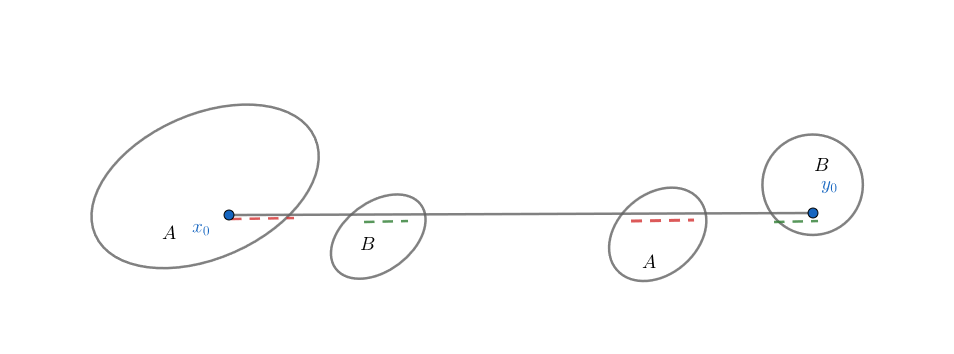
\includegraphics[width=0.5\linewidth]{Images/connectednessprof.png}
    \caption{Figure: Proof for the equivalence for connectedness for sets in $\RR$. A look at $A\cap[x_0,y_0]$ and $B\cap [x_0,y_0]$.}
    \label{fig:contced}
\end{figure}

\section{Misc Knowledge}

\thmp{}{Suppose $A_1, A_2 \cdots, A_n \cdots \in X $. Then,
\begin{enumerate}
\item If $B_n= \cup_{i=1}^n A_i$, then $\bar{B_n}=\cup_{i=1}^{n} \bar{A_i}$ 
\item $B=\cup_{i=1}^{\infty} A_i$, $\bar{B} \supseteq \cup_{i=1}^{\infty}\bar{A_i}$ with possibility of strict inequality.
\end{enumerate} }{Suppose $x \in \cup_{i=1}^{n}\bar{A_i}$. Which means
$x \in \bar{A_i}$ for some $i$. It is clear that $x$ is either a 
point of $A_i$ or a limit point of $A_i$. We have that, whatever maybe the case
either $x$ is a point in $B_n$ or a limit point of $B_n$. Therfore
$\bar{B_n}\supset \cup_{i=1}^{n} \bar{A_i}$. 
\\\\ Suppose $x$ is a point in $\bar{B_n}$. If it is a point of $B_n$,
we are done. Suppose it is the limit point of $B_n$, but not a point. Also
suppose that $x$ is not a limit point of any $A_i: i=1 \to n$. This means that,
$$\exists \varepsilon_1 \text{ such that } \forall q\in A_1, q\neq x, \text{ we have } d(q,x)\geq \varepsilon_1$$
$$\exists \varepsilon_2 \text{ such that } \forall q\in A_2, q\neq x, \text{ we have } d(q,x)\geq \varepsilon_2$$
$$\vdots$$
$$\exists \varepsilon_n \text{ such that } \forall q\in A_n, q\neq x, \text{ we have } d(q,x)\geq \varepsilon_n$$
If we choose $0<\varepsilon_0<min\{\varepsilon_i: i=1 \to n \}$, we would have that,
for every point $q$ in $A_1 \cup A_2 \cdots A_n$, $q \neq x $(which is needless to say), we have $d(q,x) \geq \varepsilon_0$ which 
makes $x$ a non-limit point of $B_n$, which is absurd. Hence we see that if $x$ is point of $B_n$ or a limit point of $B_n$, then it is a point or the limit point of some $A_j$.
\\\\ For a good counterexample, we look to $\QQ:=\{q: \text{ q is rational} \}$. This set is 
countable. Let $\{q_1, q_2, \cdots \}$ be the enumeration of $\QQ$. Consider $\QQ:=\cup_{j=1}^n \{q_j\}$. The closure
of $\QQ$ is $\RR$ but since these singleton sets are by definition closed, the union of them only gives you $\QQ$.}

\defn{Interior of a Set}{Given $S \in X$, the interior $\underbar{S}$ is defined as:
$$\underbar{S}:=\{x\in X: \exists \varepsilon_x>0 \text{ such that } B_{\varepsilon_x}(x) \subset S \} $$}
\thmp{}{The Interior is an open set}{Consider $(\underbar{S})^C:=\{x \in X: \forall \varepsilon>0, B_{\varepsilon}(x) \cap S^C \neq \phi \}$.
It is possible that $x$ is a point of $S^C$, if it is in $\underbar{S}^C$. Suppose
it is a point of $\underbar{S}^C$ but not a point of $^C$. From the definition, we see
that $\forall \varepsilon>0, \exists q \in S^C, q\neq x$ such that $d(q,x)<\varepsilon$.
This makes $x$ a limit point of $S^C$, which means, for every $x$ in $\underbar{S}^C$,
$x$ is either a point of $S^C$ or a limit point of $S^C$. Hence,
$$\underbar{S}^C \subseteq \bar{S^C} $$
Suppose $x$ is a point of $\bar{S^C}$. Say it is a point of $S^C$, then obviously,
it is a point of $(\underbar{S})^C$. Suppose $x$ is not a point of $S^C$, but a limit
point of $S^C$. This means $\forall \varepsilon>0, \exists q \in S^C, q \neq x$ so that
$d(q,x)<\varepsilon$. This is precisely the condition for which $x$ is a point of $(\underbar{S})^C$.
Hence we see $(\underbar{S})^C \supseteq \bar{(S^C)} $. Therefore, $(\underbar{S})^C=\bar{(S^C)}$. From here we 
see that $\underbar{S}$ is an open set.
\\\\ \textbf{Alternate Argument (similar):} Consider $(\underline{S})^C:=\{x \in X: \forall \varepsilon>0, B_{\varepsilon}(x)\cap S^C \neq \phi \}$
Consider a limit point $p$ of $(\underbar{S})^C$. $\forall \varepsilon>0, \exists q_{\varepsilon} \in \underbar{S}^C$ such that $d(q_{\varepsilon},p)<\frac{\varepsilon}{2} $. 
Since $q_{\varepsilon}$ is in $(\underline{S})^C$, we have that: $\forall \delta>0, \exists r_{\delta} \in S^C, r_{\delta}\neq q_{\varepsilon}$ such that $d(r_{\delta},q_{\varepsilon})<\delta$

Combining these we have:
$$(\forall \varepsilon>0)(\exists q_{\varepsilon} \in \underbar{S}^C)(\exists \delta>0)(\exists q_{\delta} \in S^C)$$
$$(d(q_{\delta},p)\leq d(q_{\delta},q_{\varepsilon})+d(q_{\varepsilon},p)<\frac{\varepsilon}{2}+\delta<\varepsilon) $$
This means $p$ is a limit point of $S^C$. Hence, $\underbar{S}^C$ is closed.}
\thmp{}{$\underbar{S}=S$ $\iff$ $S$ is open}{$\implies $) if $\underbar{S}=S$, obviously 
$S$ is open.
\\\\ $\impliedby)$ If $S$ is open, then by definition $\underbar{S}=$ set of all
points in $S$ so that there's an $\varepsilon$-ball of $x$ in $S$. But that is every point
of $S$. }
\thmp{}{$\underbar{S}$ is the largest open set contained in $S$}{Consider an open
subset of $S$. These are subsets of $S$ whose each point has an $\varepsilon$-ball
around it so that the ball is contained in the subset, which is contained in $S$. So by 
definition, these points in these subsets are contained in $\underbar{S}$.}
\thmp{}{$$(\underbar{S})^C=\overline{(S^C)}$$ \centering{"The compliment of the interior is the closure of the compliment"}}{Refer to the proof of "Interiors of sets are Open", to see this construction.
\\\\ \textbf{Alternate method(slicker):}
\\\\ $\underbar{S} \subseteq S\implies S^C \subset (\underbar{S})^C$ where $(\underbar{S})^C$
is a closed set containing $S^C$. Since $\overline{S^C}$ is the smallest closed set that contains $S^C$, we
have $\overline{S^C} \subseteq (\underbar{S})^C $.
\\\\ Note that $S^C \subseteq \overline{S^C} \implies (\overline{S^C})^C \subseteq S$ where $(\overline{S^C})^C$
is an open set inside $S$. Since $\underline{S}$ is the largest open set containing $S$,
we have that $ (\overline{S^C})^C \subseteq \underline{S} \implies \underline{S}^C \subseteq \overline{S^C}$. Combining these
two set inequalities, we are done.
}

\thmp{}{\begin{enumerate}
\item If $A$ and $B$ are closed, disjoint subsets of $X$, then $A$ and $B$ are separated.
\item If $A$ and $B$ are open, disjoint sets, then $A$ and $B$ are separated.
\end{enumerate} }{(1) $A$ $B$ closed implies $A=\overline{A}$ and $B=\overline{B}$ which are disjoint. From here it is obvious.
\\\\ (2) $A$ and $B$ are open disjoint sets, then we see that $A \subseteq B^C $ and $B \subseteq A^C$ where 
$A^C$ and $B^C$ are closed by definition. Since closure is the smallest closed set containing $A$ (and $B$), we see that $\overline{A} \subseteq B^C$ and $\overline{B}\subseteq A^C$.
It is now trivial to see that $\overline{A}\cap B \subseteq B^C \cap B=\phi=\overline{B}\cap A $ which is the definition of separated.
}
\corp{Let $p\in X$ and $\delta>0$. Define $A:=B_{\delta}(p)$ and $B=(B_{[\delta]}(p))^C$. $A$ and $B$ are, then, separeted. }{Easy to see that they are both open sets that are disjoint.}{}

\thmp{}{Every connected metric space with atleast two points is uncountable.}{Let $a$ and $b$ be in $X$. Let $\xi\leq d(a,b)$. 
Note that, $P=B_{\xi}(a)$ and $Q=(B_{[\xi]}(a))^C$ are non empty, separated sets (from the previous corollary).
If $X$ is not the union of $P$ and $Q$, then there is a point $z_{\xi}$ in $X$ so that it is neither in $P$
not in $Q$. That means that it is exactly $\xi$ distance away from $p$. For every $\xi<d(a,b)$,
there exists a point $z_{\xi}$ so that its distance from $p$ is exactly $\xi$. Therefore, every $z_{\xi}$ 
is unique (from positivity property of metric spaces) which means there are uncountable $z_{\xi}$-s.
}

\thmp{}{If $P$ and $Q$ are connected such that $P \cap Q \neq \phi$, then $P \cup Q$ is also connected.}{Suppose $P \cup Q$ is actually not connected. This means $P \cup Q= A \cup B$ for non empty, separated sets $A$ and $B$. Suppose $P$ is fully contained in $A$. This means that $Q$ has intersection with $A$ and intersection with $B$ which are non empty. Obviously $Q \subseteq A \cup B$ which means $Q= (A \cap Q)\cup(B \cap Q)$ where $(A \cap Q)$ and $(B \cap Q)$ are separated and non empty. Since $Q$ is connected, this is absurd. Suppose then that $P$ is not fully contained in $A$. This means that $P \cap A$ and $P \cap B$ is non empty each. This means $P=(P \cap A) \cup (P \cap B)$. From the same reasoning, this is absurd.}

\lemp{}{Given two balls $B_1$ and $B_2$ in $\RR^n$ that are closed, with $B_1 \cap B_2=\{z\}$ with $z \in \RR^n$, then the interior of $B_1 \cup B_2$, i.e, $\underline{B_1 \cup B_2}$, is $\underline{B_1} \cup \underline{B_2}$, which are their respective open ball counterparts.}{We understand that $\underline{B_1} \cup \underline{B_2} \subseteq \underline{B_1 \cup B_2}$. Note that none of the "rim" points of $B_1$ or $B_2$, are in the interior. This would conclude the result.}

\corp{If $A \subset X$ is connected, it needn't be true that $\underline{A}$ is connected.}{Consider the set $B_1 \cup B_2$ from the previous lemma. We note that, its interior is the disjoint union of two non empty open balls. These two sets are separated, which makes $\underline{B_1 \cup B_2}$ a separated set.}{}

\thmp{}{Let $E$ be the set of all $x \in [0,1] \subseteq \RR$ so that the decimal expansion of $x$ only contains $4$ and $7$. Then:
\begin{enumerate}
\item $E$ is uncountable
\item $E$ is not dense in $[0,1]$
\item $E$ is compact
\item $E$ is prefect
\end{enumerate}
}{(1) $E$ is uncountable via the diagonal argument. If $\{x_1,x_2,\cdots \}$ is the enumeration of $E$, simply take the first decimal place of $x_1$ and flip it (i.e. to $4$ if $7$ or vice versa). Likewise for $x_2$ and so on to get a new decimal expansion that is unlike all $x_1,x_2\cdots x_n \cdots$ which is a contradiction.
\\\\ (2) Obviously, since $0.4 \leq x \leq 0.8$ for any $x\in E$.
\\\\ (3) We already know $E$ is bounded. Consider $E^c$. This is the set of all numbers in $[0,1]$ so that not all points in the decimal expansion is $4$ or $7$. i.e, there would be a point in the expansion that is neither $4$, nor $7$. Suppose we take one such arbitrary $x \in E^c$. Let the first non $4,7$ number occur at the $j-$th place. $0.z_1z_2z_3\cdots x_j \cdots $. Look for another non $4,7$ after the $j-$th place (if it exists). If it doesn't exist, then all the numbers after $x_j$ would be $4$ or $7$ so safely add $10^{-(j+1)}$ as our $\varepsilon$. This $\varepsilon$ range around $x$ would contain only points of $E^c$. Suppose another point exists that is non $4,7$ after $j$, perhaps at $k>j$-th index. Then it would look something like:
$0.z_1z_2 \cdots z_jx_{j+1}x_{j+2} \cdots z_k \cdots$. Here we simply take $\varepsilon=10^{-(k+1)}$ so that all points in the $\varepsilon$-neighbourhood of $x$ is in $E^c$. Therefore, $E^c$ is open, which means $E$ is closed. Closed and bounded implies compact in $\RR$.
\\\\ We saw that $E$ is closed. We need only show that every point of $E$ is a limit point of $E$. This can be done easily for any $\varepsilon$-ball, using the technique that follows:
Choose a $k$ so that $\frac{1}{10^k}<\varepsilon$. Look at the interval $x-\frac{1}{10^k},x+\frac{1}{10^k}$ that is contained in $E$. Just find some $n>k$, and flip the $4$ to a $7$ or vice versa to land in a "different" element from $x$, yet within the neighbourhood in consideration. Hence, every point is a limit point, making $E$ a perfect set.

}

\thmp{Existence of a compact set in $\RR$ with countable limit points.}{Title}{Consider the points $x_1=1, x_0=0, x_2=\frac{1}{2}, \cdots x_{n}=\frac{1}{n} \cdots$. Let $x_{11}<x_{12} \cdots <x_{1n}$ be a sequence that converges to $x_1=1$. Let $x_{21}<x_{22}<x_{23} \cdots <x_{2n} \cdots $ be a sequence convergent to $x_2=\frac{1}{2}$, with the added condition that $x_{2j} < x_{1k}$ for every $j,k \in \NN$. Likewise for every $x_n$, create a sequence $x_{nk}$ that converges to $x_n$. Make sure that $x_{an}<x_{bm}$ if $a>b$, for every $m,n$. We therefore have:
$$x_{11}<x_{12}\cdots \to x_1 $$  
$$x_{21}<x_{22}\cdots \to x_2$$
$$ \vdots$$
We claim that the set $\Phi=$ $x_0,x_1,x_2, \cdots$ along with $x_{11},x_{12}\cdots, x_{21},x_{22}\cdots x_{n1}$ etc. forms a Compact set in $\RR$ that has countable limit points. 
\\\\ Suppose that $q \in \RR \neq 0$ and $q \neq \frac{1}{j}$ for any $j$ be a limit point of $\Phi$. This means a subsequence $z_n$ in $\Phi$ converges to $q$. Does infinite points of $x_{1j}$ exist in the subsequence $z_n$ convergent to $q$? Obviously not, since that would make a subsequence of $z_n$ convergent to one of $1$. So only utmost finite elements of $x_{1j}$ are in $z_n$. Same way one can argue that utmost finite elements of $x_{kj}$ are in $z_n$ for every $k$. If we establish a subsequence of $z_n$ that converges to $0$, then the only limit point of $\{z_n\}$ would be $0$ which would mean $0$ is where $z_n$ would converge. Enough wishful thinking; Does any point of $x_{1j}$ exist in $z_n$? If yes, choose that point. If not, find the next $n_1$ so that a point in $x_{n_1 j}$ is in $z_n$. Find, then $n_2>n_1$ so that some point in $x_{n_2 j}$ is in $z_n$. As such keep going, making $n_1<n_2<\cdots$ and a sequence that is monotone decreasing by construction, that converges to $0$. Hence, this is a subsequence in $\{z_n\}$ that converges to $0$. If $z_n$ converged to $q$, then the only limit point would be $q$. Hence, $q=0$. This means that the only limit points of $\Phi$ other than $\frac{1}{j}$ is $0$. Hence, we have a countable limit point. Hence, $\Phi$ is a closed set and bounded obviously, with countable limit points. }

\thmp{technique weve already seen}{If $A$ and $B$ are separated sets in $\RR^n$ (that are non empty), and $\vec{x_0} \in A$ and $\vec{y_0} \in B$, define $p(t)=\vec{x_0}+t(\vec y_0 -\vec x_0)$ for $t\in [-\infty,\infty]$ and $$S_A:=\{ t \in \RR: p(t) \in A \} $$ $$S_B:=\{t \in \RR: p(t) \in B \} $$ Then:
\begin{enumerate}
    \item $S_A$ and $S_B$ are separated sets
    \item $\exists t_0 \in (0,1)$ so that $t_0 \not\in S_A \cup S_B$
\end{enumerate}
}{(1) If $S_A$ and $S_B$ weren't disjoint, then obviously $A$ and $B$ wont be. If there is a sequencei n $S_A$ converging in $S_B$ or vice-versa, it is easy to see that this would lead to there exiting a sequence in $A$ converging to $B$ (or vice-versa). Therefore, $S_A$ and $S_B$ are separated.
\\\\ (2) Since $S_A$ and $S_B$ are separated and non-empty, there are two points $x_0$ and $y_0$ in $S_A$ and $S_B$ respectively. Define $z(l)=x_0+l(y_0-x_0)$ for $l \in [0,1]$. Now, for some $l_A$, we have that for every $l>l_A$, $z(l) \not\in S_A$, the set $G_A:=\{l: z(l) \in S_A \}$ is therefore bounded above with supremum $u_A$. Likewise for some $l_B$, we have that for every $l<l_B$, $z(l) \not\in S_B$, the set $G_B:=\{l: z(l) \in S_B \}$ is therefore bounded below with infimum $v_B$. Note that $G_A$ and $G_B$ are separated sets. We may as well assume that for every $l<l_B$, $l$ is in $G_A$, or $z(l)$ falls in $S_A$. If not, we would be done. We now ask: does $v_B$ fall in $G_A$ or $G_B$? If it falls in $G_B$, there exists a sequence in $G_A$ that would converge to $v_B$, which is absurd. If it falls in $G_A$, then by virtue of being the infimum of $G_B$, there is a sequence in $G_B$ converging in $G_A$. Hence, there exists a point $l$ between $x_0$ and $y_0$ $l \not\in G_A$ or $G_B$ which means $z(l) \not \in S_A$ or $S_B$. This again means that $p(z(l)) \not \in A$ or $B$. Phew.   
}

\corp{Every convex set in $\RR^n$ is connected.}{If they were not connected, then there would exist sets $A$ and $B$, non empty, disjoint and separated so that our convex set $C$ would be $A \cup B$. Suppose $x_0 \in A$ and $y_0 \in B$. From the previous theorem we see that, if $z(t)=x_0 +t(y_0-x_0)$, then there would exist $t'$ so that $z(t') \not\in A $ or $B$, which means it wont be in $C$. But if $x_0$ and $y_0$ are in $C$, by definition of convexity, $z(t)$ for any $t$ must exist in $C$. Contradiction. }{}

\exm{A Pedagogical Example.}{If $E:=\{ q \in \QQ: 2<q^2<3\}$ is considered a set in the metric subspace of $\QQ$ with the usual distance, then we have:
\begin{enumerate}
    \item $E$ is closed and bounded (wrt $\QQ$ obviously)
    \item $E$ is \emph{non compact}.
    \item $E$ is open with respect to $\QQ$
\end{enumerate} 
\begin{proof}
Consider an arbitrary convergent sequence $p_n$ in $E$. We see that if $p_n$ is contained in $E$, then $2<p_n^2<3$. If we pass to the limit, we would have $2 \leq q^2 \leq 3$ but the limit $q$ would either not exist in $\QQ$ (whence the sequence $p_n$ wouldn't be convergent anyway) or it does, in which case it follows $2<q^2<3$ (since no rational number has its square as $2$ or $3$). Therefore, we can see that every convergent sequence in $E$ converges in $E$. Hence, $E$ is closed. Boundedness is obvious.
\\\\ One way to see that $E$ is non compact is simply by making use of the "conservation" of compactness going from one space to a bigger space or vice-versa. Since $E$ is clearly not compact in $\RR$, it wont be compact in the metric subspace $\QQ$. Another way to see that it is non compact is to consider the following construction:
Look at the union of the two split intervals $(-\sqrt{3},-\sqrt{2})$ and $(\sqrt{2},\sqrt{3})$. Let $h=\sqrt{3}-\sqrt{2}$. We construct it for the right side interval, and simply copy it to the left one. Choose the point $\sqrt{3}$ and a $h/2$-ball around $\sqrt{3}$ and call it $V_0$. This would intersect the right interval at a distance $h/2$ from $\sqrt{3}$. Choose this intersection point and a $h/4$-ball around this called $V_2$. Both $V_1$ and $V_2$ together covers $3h/4$ of the interval. Choose this intersection point and let the $h/8$-ball around this point be $V_3$. $V_1$, $V_2$ and $V_3$ together cover $7h/8$ of the interval. Keep going as such to construct $V_n$ so that $(V_i)_{i=1}^n$ covers $\frac{(n-1)h}{n}$ of the whole interval. As $n$ tends to $\infty$, the "coverage" converges to $h$. This means that for every $\varepsilon$ distance away, there exists a finite $n_0$ so that $V_1 \to V_{n_0}$ covers up to that $\varepsilon$ distance. Every point $e$ in the strict interval would therefore be covered up by some $V_k$ by our construction. But obviously, this "open cover" has no finite subcover, for no finite "coverage" covers all the way till $h$ distance of the interval. Some $\varepsilon$-gap is always left, hence missing points.
\\\\ $E$ can also be written as the disjoint union of the set $A$ of all $p$ so that $\sqrt{2}<p<\sqrt{3}$ and the set $B$ of all $p$ so that $-\sqrt{3}<p<-\sqrt{2}$. WLOG say $q \in A$. Obviously $\sqrt{2}<q<\sqrt{3}$. Choose $\delta< min\{\sqrt{3}-q, q-\sqrt{2}\}$ and the $\delta-$ball called $V$ around $q$. Easy to see that this ball $V$ is fully contained in $A$. Likewise, it can be shown for $B$ as well. Hence, $E$ is open with respect to $Q$. 
\end{proof}

}

\end{document}
